\documentclass{sig-alternate-05-2015}

%% =============================================================
% \def\tool{\textsc{Tool}\xspace}
% \def\papertitle{\tool: Memory-Efficient and Time-Bounded Runtime Monitoring for 
% Resource-Constrained Systems}
\def\papertitle{Efficient and Context-Aware Finite-State Runtime Monitoring}
\def\pdfauthors{}
\def\paperkeywords{}
%% =============================================================

%------------------------------------------------------------------------------
%                                Pre-package misc.
%------------------------------------------------------------------------------

\usepackage{color}

\interfootnotelinepenalty=10000
\sloppy

% You can tweak clickable link colors here:
\definecolor{linkcol}{rgb}{0,0,1}
\definecolor{citecol}{rgb}{0,0.5,0}
\definecolor{urlcol}{rgb}{0.3,0,0}

% Make pdflatex use letter size --md
\setlength{\pdfpagewidth}{8.5in}
\setlength{\pdfpageheight}{11in}

%------------------------------------------------------------------------------
%                                Use packages.
%------------------------------------------------------------------------------

\usepackage{tikz}
\usepackage{amsmath}
\usepackage{ragged2e}
\usepackage{cite}
\usepackage{txfonts}
\usepackage{fancyhdr}
\usepackage{amssymb}
\usepackage{fancyvrb}
\usepackage{graphicx}
\usepackage{times}
\usepackage{pifont}
\usepackage{xspace}
\usepackage{epstopdf}
%%\usepackage[belowskip=-10pt,aboveskip=5pt,small,labelfont=bf]{caption}
\usepackage[aboveskip=5pt,small,labelfont=bf]{caption}
\usepackage{subcaption}
% \usepackage[hyphens]{url}
\usepackage{url}

\DeclareCaptionType{copyrightbox}

\usepackage[bookmarks=true,%
bookmarksnumbered=true,%
colorlinks=true,%
linkcolor=linkcol,%
citecolor=citecol,%
urlcolor=urlcol,%
hypertexnames=true,%
pdfpagelabels]{hyperref}

% \usepackage{sty/algorithm2e}
\usepackage{sty/multirow}
% \usepackage{sty/flushend}
% \usepackage{sty/usenix}
\usepackage{sty/epsfig}
\usepackage{sty/endnotes}
\usepackage{sty/algorithm} 
\usepackage{sty/algorithmic}
% \usepackage{sty/listings}

\newcommand{\subparagraph}{}
\usepackage[small,compact]{sty/titlesec}

%------------------------------------------------------------------------------
%                                Space savers.
%------------------------------------------------------------------------------

% \SetAlFnt{\small}
% \SetAlCapFnt{\small}
% \SetAlCapNameFnt{\small}
%%\SetVlineSkip{0pt}

\setlength\floatsep{5pt}
\setlength\textfloatsep{5pt}
\setlength\intextsep{5pt}

% Use a smaller font size for URLs:
\makeatletter
\def\url@myurlstyle{%
   \@ifundefined{selectfont}{\def\UrlFont{\small}}{\def\UrlFont{\small}}}
   \makeatother
\urlstyle{myurl}

%------------------------------------------------------------------------------
%                                Misc.
%------------------------------------------------------------------------------

% This adds ':' to the characters after which not to break URLs, and
% defines a smaller typewriter font. --cpk
% changed small to sf -- md
\def\UrlNoBreaks{\do:\do\(\do\[\do\{\do\<}%
\def\UrlFont{\small\ttfamily}
\def\UrlOrds{\do\*\do\~}%

% For referencing sections, Vern-style
\newcommand\xref[1]{\S~\ref{#1}}

\newcommand\fref[1]{Fig.~\ref{#1}}

% Black filled circles with white number on it
% See Comprehensive LaTeX Symbol List --cpk
\def\blackI{\ding{182}}
\def\blackII{\ding{183}}
\def\blackIII{\ding{184}}
\def\blackIV{\ding{185}}
\def\blackV{\ding{186}}
\def\blackVI{\ding{187}}

\def\first{({\it i})\xspace }
\def\second{({\it ii})\xspace }
\def\third{({\it iii})\xspace }
\def\fourth{({\it iv})\xspace }
\def\fifth{({\it v})\xspace }

% For notes to authors:
\newcommand{\note}[1]{{\textcolor{red}{[\textit{#1}]}}}

% Fine-tuning for table spacing. --cpk
\def\TblSpT{\rule[-1ex]{0pt}{0pt}}
\def\TblSpB{\rule{0pt}{2.5ex}}

% Squeezing out some space. --cpk
% http://www-h.eng.cam.ac.uk/help/tpl/textprocessing/squeeze.html
%
%\renewcommand\subfigtopskip{0pt}
%\renewcommand\subfigbottomskip{5pt}
%\renewcommand\subfigcapskip{0pt}
%\renewcommand\floatpagefraction{.9}
%\renewcommand\topfraction{.9}
%\renewcommand\bottomfraction{.9}
%\renewcommand\textfraction{.1}
%\setlength{\parskip}{0em}
%\frenchspacing

%------------------------------------------------------------------------------
%                                Space savers.
%------------------------------------------------------------------------------
% This mylist environment indents items, and saves less space than the above.
\newcounter{myctr}
\newenvironment{mylist}{\begin{list}{(\textbf{\arabic{myctr}})}
{\usecounter{myctr}
\setlength{\topsep}{1mm}\setlength{\itemsep}{0.5mm}
\setlength{\parsep}{0.5mm}
\setlength{\itemindent}{0mm}\setlength{\partopsep}{0mm}
\setlength{\labelwidth}{-2mm}
\setlength{\leftmargin}{0mm}}}{\end{list}}


\newcounter{myctr1}
\newenvironment{challenges}{\begin{list}{\textbf{C\arabic{myctr1}.}}
{\usecounter{myctr1}
\setlength{\topsep}{1mm}\setlength{\itemsep}{0.5mm}
\setlength{\parsep}{0.5mm}
\setlength{\itemindent}{0mm}\setlength{\partopsep}{0mm}
\setlength{\labelwidth}{-2mm}
\setlength{\leftmargin}{0mm}}}{\end{list}}

% Space saving List environment for itemizing.
\newenvironment{mybullet}{\begin{list}{$\bullet$}
{\setlength{\topsep}{1mm}\setlength{\itemsep}{0.5mm}
\setlength{\parsep}{0.5mm}
\setlength{\itemindent}{0mm}\setlength{\partopsep}{0mm}
\setlength{\labelwidth}{-2mm}
\setlength{\leftmargin}{0mm}}}{\end{list}}

\newcommand{\myparagraph}[1]{\noindent{\scshape \bfseries #1.}}

%------------------------------------------------------------------------------
%                               Fancy header setup.
%------------------------------------------------------------------------------
%
\pagestyle{fancyplain}
\lhead{}
\lfoot{}
\chead{}
\rhead{}
\cfoot{\thepage}
%%\rfoot{{\scriptsize \today}}
\renewcommand{\headrulewidth}{0pt}

%\setlength{\intextsep}{10pt plus 2pt minus 2pt}

%% Reducing margins further -- md
%%\addtolength{\hoffset}{-0.25in}
%%\addtolength{\textwidth}{0.5in}
%%\addtolength{\voffset}{-0.25in}
%%\addtolength{\textheight}{0.4in}

%------------------------------------------------------------------------------
%                                New commands
%------------------------------------------------------------------------------

\newcommand{\code}[1]{\texttt{\small{#1}}}
% \newcommand{\code}[1]{\texttt{\scriptsize{#1}}}
\newcommand{\mycomment}[1]{}
\newcommand{\ignore}[1]{}
\newcommand{\todo}[1]{\textbf{TODO: #1}}
\newcommand{\mytab}{~~~~}
\newcommand{\sspace}{~}
\newcommand{\etal}{\textit{et al.}}
\newcommand{\eg}{{e.g.,}}
\newcommand{\ie}{{i.e.,}}
\newcommand{\lno}[1]{{\tiny{\textbf{(#1)~~}}}}
\newcommand{\packetin}{\code{PACKET\_IN}}
\newcommand{\flowmod}{\code{FLOW\_MOD}}
\renewcommand{\put}{\code{PUT}}
\newcommand{\delete}{\code{DELETE}}
\newcommand{\post}{\code{POST}}
\newcommand{\get}{\code{GET}}
\newcommand{\head}{\code{HEAD}}
\newcommand{\rest}{\textsc{rest}}
\newcommand{\rpc}{\textsc{rpc}}

\newcommand{\docker}{Docker}
\newcommand{\tikzcircle}[3][black,fill=white]{\tikz[baseline=-0.75ex]\draw[#1,
radius=#2] (0,0) circle node[text=black] {\scriptsize #3};}%
%%\newcommand*\circled[1]{\tikz[baseline=(char.base)]{\node[shape=circle,draw,
%%inner sep=2pt] (char) {#1};}}
\newcommand{\rulesep}{\unskip\ \vrule\ }
% \newcommand{\sdn}{{SDN}}
% \newcommand{\verifier}{\textsc{Verifier}}
% \newcommand{\validator}{\textsc{Flow\_Consistency\_ Validator}}
% \newcommand{\outputs}{{\mathbb O}}
% \newcommand{\stream}{{\mathbb S}}
% \newcommand{\os}{OpenStack}

% \SetEndCharOfAlgoLine{}

\renewcommand{\thetable}{\arabic{table}}

%\newcommand*{\refname}{Bibliography}

\def\yes{\ding{51}}
\def\no{\ding{55}}

% The space-saving sledgehammer. -- md
%\renewcommand{\baselinestretch}{0.95}

\hypersetup{
pdfauthor = {},
pdftitle = {\papertitle},
pdfkeywords = {\paperkeywords},
pdfcreator = {LaTeX with hyperref package},
pdfproducer = {pdflatex}}


%% only for the tech report
%%\makeatletter
%%\def\@copyrightspace{\relax}
%%\makeatother

\begin{document}

% Copyright
\setcopyright{acmcopyright}
%\setcopyright{acmlicensed}
%\setcopyright{rightsretained}
%\setcopyright{usgov}
%\setcopyright{usgovmixed}
%\setcopyright{cagov}
%\setcopyright{cagovmixed}

% DOI
\doi{10.475/123_4}

% ISBN
\isbn{123-4567-24-567/08/06}

%Conference
\conferenceinfo{ISSTA '16}{July 17--20, 2016, Saarbrucken, Germany}

\acmPrice{\$15.00}

% %
% % --- Author Metadata here ---
% \conferenceinfo{WOODSTOCK}{'97 El Paso, Texas USA}
% %\CopyrightYear{2007} % Allows default copyright year (20XX) to be over-ridden - 
% IF NEED BE.
% %\crdata{0-12345-67-8/90/01}  % Allows default copyright data 
% (0-89791-88-6/97/05) to be over-ridden - IF NEED BE.
% % --- End of Author Metadata ---

\title{\Large \bf \papertitle}

% % ISSTA'16 is double blind, so removed the author block

\maketitle

\begin{abstract}
%%
\small

% % Runtime monitoring is employed in practice to ensure that a program shows 
% % expected behavior during its execution. Past decade has seen a prominent rise in 
% % the number of novel runtime monitoring frameworks and tools due to the promise 
% % shown by monitoring techniques. Many of these tools have been used effectively 
% % to verify typestate properties that are associated with legal Application 
% % Programming Interface (API) usages. In spite of their effectiveness, the tools 
% % have been occasionally found to incur significant runtime overheads, which could 
% % be even larger than the program's own execution time, particularly when the 
% % properties are associated with multiple objects. Moreover, the overheads have 
% % also been found to be extremely variable even when handling the events of the 
% % same kind. Such undesirable overheads may restrict the application of monitoring 
% % only to test environments or even worse, make it infeasible. In addition to time 
% % overheads, the monitoring tools also consume significant memory to keep 
% % monitors. 

% % Occasionally this extra memory outweighs the program's own memory requirements. 
% % All of these limitations make runtime monitoring infeasible for real-time 
% % programs that are typically executed in resource-constrained environments, where 
% % functional as well as non-functional requirements are critical.In this work, we 
% % propose a monitoring framework that investigates the trade-off between the 
% % runtime overhead and the error reporting. Our approach is motivated by the fact 
% % that there is a large redundancy among monitors in terms of their behavior which 
% % results in many monitors detecting same errors. The approach works by limiting 
% % the number of monitors based on heuristics that are related to the program 
% % execution context. In addition, the approach also limits the number of monitors 
% % that are associated with events related to a set of objects. As a result, the 
% % framework enables monitoring which consumes much less memory and provides 
% % worst-case bounds for the execution times of handling events. Moreover, our 
% % study based on some challenging typestate properties and DaCapo benchmarks 
% % indicates that our approach does not result in extra memory overhead. At the 
% % same time, it detects all the violations that an un-optimized approach detects.

Runtime monitoring is employed in practice to ensure that a program shows 
expected behavior during its execution. However, monitoring has been 
occasionally found to incur large and unpredictable overheads in terms of memory 
and time, which makes its application challenging in resource-constrained 
environments. Past research has shown that this challenge is particularly big 
when the properties the programs are monitored for are finite state, 
parameterized, and associated with objects that are created in large numbers. In 
this work, we propose a novel monitoring approach that investigates various 
trade-offs associated with memory overhead of monitoring, the execution times of 
monitoring operations, and the error reporting, which are key attributes of 
resource-constrained systems. Our approach is motivated by two key observations. 
First, there is prominent behavioral redundancy among monitors resulting in more 
than one monitors detecting same errors. Second, there is a temporal separation 
among monitored events that belong to distinct monitors. We leverage these 
observations to reduce the number of monitors, and provide compact worst-case 
time bounds to monitoring operations, without compromising much with the 
soundness of the optimized monitoring system. Evaluation of our prototype 
implementation using challenging combinations of finite state properties and 
DaCapo benchmarks indicates that our approach can effectively control the memory 
overhead and worst-case execution times without adding extra runtime overhead.

%%
\end{abstract}

\begin{CCSXML}
<ccs2012>
 <concept>
  <concept_id>10010520.10010553.10010562</concept_id>
  <concept_desc>Computer systems organization~Embedded systems</concept_desc>
  <concept_significance>500</concept_significance>
 </concept>
 <concept>
  <concept_id>10010520.10010575.10010755</concept_id>
  <concept_desc>Computer systems organization~Redundancy</concept_desc>
  <concept_significance>300</concept_significance>
 </concept>
 <concept>
  <concept_id>10010520.10010553.10010554</concept_id>
  <concept_desc>Computer systems organization~Robotics</concept_desc>
  <concept_significance>100</concept_significance>
 </concept>
 <concept>
  <concept_id>10003033.10003083.10003095</concept_id>
  <concept_desc>Networks~Network reliability</concept_desc>
  <concept_significance>100</concept_significance>
 </concept>
</ccs2012>  
\end{CCSXML}

\ccsdesc[500]{Computer systems organization~Embedded systems}
\ccsdesc[300]{Computer systems organization~Redundancy}
\ccsdesc{Computer systems organization~Robotics}
\ccsdesc[100]{Networks~Network reliability}


%
% End generated code
%

%
%  Use this command to print the description
%
\printccsdesc

% We no longer use \terms command
%\terms{Theory}

\keywords{monitoring, memory optimization, boundedness, scalability, reuse}
\section{Introduction}
\label{sec:introduction}

Modern software applications are complex and diverse in nature. They come in 
various forms ranging from large web-based systems that serve large number of 
user requests in reasonable time to applications that run on small hand-held 
mobile devices. Irrespective of their forms, they pose challenges for tools that 
perform automatic verification either statically or dynamically. Even though 
useful, static analysis techniques often produce numerous false positives 
that are hard to analyze~\cite{Deline04,Naeem:ECOOP08}, or need
annotations from developers~\cite{Bierhoff:ECOOP09, Bierhoff:OOPSLA07} which puts
an extra burden on them. Hence, researchers have invested time and 
effort to develop runtime monitoring tools and techniques that are precise
and can scale to realistic programs \cite{Allan:OOPSLA05, Arnold:OOPSLA08, chen2005, Reger2015}.

In spite of their effectiveness, monitoring tools have been occasionally found 
to incur considerable memory and execution overheads making their deployment 
challenging even
% in production or even 
test environments ~\cite{Purandare:2013}.
% challenging. 
Monitoring can often consume memory and compute resources 
% that are even 
greater than those 
% the ones 
consumed by the monitored program itself,
% being monitored 
especially when properties of interest are complex and are associated with objects 
generated in large numbers, such as collections and iterators~\cite{chen2009}. 
Monitoring overhead can be a big concern considering that in practice 
programmers would like to track several properties at a time, which cumulatively 
adds the overheads of individual properties~\cite{luo-2014, Purandare:2013}.

The monitoring overheads are unpredictable since they depend on the program and 
property interactions. For a given program and property, the interactions depend 
on the executed program paths. To make matters worse, 
monitoring operations corresponding to an event may take arbitrarily long when 
the properties are associated with multiple objects.
These operations can consume variable 
execution times even for similar events owing to the fact that variable number 
of monitors may be associated with each one of those events at different times
and each one of the 
monitors needs to be tracked after the occurrence of these events. This number 
can grow rapidly and is theoretically unbounded. In one study, up to 1548 monitors
associated with a single object have been reported ~\cite{Purandare:2013}.

Large and unpredictable overheads pose serious challenges to monitoring since 
they adversely impact the system performance.
%For real-time embedded 
%applications, developers need to provide bounds for the worst case execution 
%times of system operations.
%As a result, the usage of runtime monitoring is 
%restricted either to testing environments or to the production environments in 
%which resources are abundant and performance requirements are less stringent. 
Even though resource-constrained systems such as mobile and real-time embedded 
systems have more restrictive resource requirements, all modern systems 
including
% the embedded as well as many
web-based and cloud-based systems have practical constraints on their resources 
considering that the applications they run are often CPU- and memory-intensive, 
and their performance is expected to be high and predictable. Hence, in order to 
employ runtime monitoring in production environment, we need novel and efficient 
techniques that consume less resources and provide guarantees about their 
performance. At the same time, the techniques should also be effective in 
catching property violations, which is the primary objective of runtime 
monitoring.

Researchers have tried several approaches in the past, and developed tools to 
monitor programs efficiently by keeping the overall overheads within limits by 
turning off monitoring if it exceeded the allocated time
budget~\cite{Arnold:OOPSLA08, BartocciGKSSZS12, StollerBSGHSZ11}. 
However, these approaches do not deal with the properties that are related to 
multiple objects, and do not give guarantees about the worst-case execution 
times of monitoring operations. Moreover, they do not directly control the 
memory overheads. Other approaches either do not deal with finite-state 
properties or not perform inline monitoring. Finite state property 
monitoring allows us to check programs for properties that are more expressive, 
whereas inline monitoring allows us to keep the detection latency within limits, 
and also provides opportunities for performing evasive actions avoiding 
failures~\cite{DwyerPP10}.

In this work, we propose a novel inline monitoring technique that investigates 
the trade-off between limited resources, namely memory and monitor execution 
times, and the error reporting. Our approach is motivated by a key 
observation that there is large redundancy among monitors in terms of their 
behavior that results in many monitors detecting the same error. However, 
programmers are interested in catching distinct errors, rather than several 
instances of the same error. Our technique works by limiting the number of 
monitors based on heuristics related to the program's execution context. When 
the properties are related to multiple objects, there can be several monitors 
waiting for an event. Since the number of these monitors is unbounded, the 
technique puts a hard limit on the number of monitors associated with the 
event. As a result, 
it consumes much less memory and provides tight worst-case bounds on the 
execution times of handling events.

The second key observation that we make is about the occurrence of events.
We observe that he events on the same or related objects often occur together
and are temporally separated from the rest. As a consequence, we observe
that newly created objects are likely to be associated with recent events.
We make use of these observations to develop heuristics to prioritize monitors
in the allocation to maintain the soundness of the system.

%Our study based on some challenging finite-state properties and DaCapo benchmarks 
%indicates that the technique has a potential to detect all distinct violations that an 
%un-optimized approach could detect. Moreover it can detect these violation using
%much less resources in terms of memory and execution time.

This paper makes two major contributions.
% of our research is double-fold. 
First, we present a novel approach~\xref{sec:approach} that is memory-efficient 
and time-deterministic. Second, we present a study of a prototype 
implementation~\xref{sec:implementation} of our approach on realistic 
benchmarks and properties. Our evaluation~\xref{sec:evaluation} based on some
challenging Java standard library properties and DaCapo benchmarks 
indicates that the technique has a potential to detect all distinct violations that an 
un-optimized approach could detect. Moreover it can detect these violation using
much less resources in terms of memory and execution time.


%indicates the effectiveness of our approach.

\ignore{Runtime monitoring is employed in practice to ensure that a program 
shows expected behavior during its execution. Past decade has seen a prominent 
rise in the number of novel runtime monitoring frameworks and tools due to the 
promise shown by monitoring techniques. Many of these tools have been used 
effectively to verify typestate properties that are associated with legal 
Application Programming Interface (API) usages. In spite of their effectiveness, 
the tools have been occasionally found to incur significant runtime overheads, 
which could be even larger than the program's own execution time, particularly 
when the properties are associated with multiple objects. Moreover, the 
overheads have also been found to be extremely variable even when handling the 
events of the same kind. Such undesirable overheads may restrict the application 
of monitoring only to test environments or even worse, make it infeasible. In 
addition to time overheads, the monitoring tools also consume significant memory 
to keep 
monitors. Occasionally this extra memory outweighs the program's own memory 
requirements. All of these limitations make runtime monitoring infeasible for 
real-time programs that are typically executed in resource-constrained 
environments, where functional as well as non-functional requirements are 
critical.In this work, we propose a monitoring framework that investigates the 
trade-off between the runtime overhead and the error reporting. Our approach is 
motivated by the fact that there is a large redundancy among monitors in terms 
of their behavior which results in many monitors detecting same errors. The 
approach works by limiting the number of monitors based on heuristics that are 
related to the program execution context. In addition, the approach also limits 
the number of monitors that are associated with events related to a set of 
objects. As a result, the framework enables monitoring which consumes much less 
memory and provides worst-case bounds for the execution times of handling 
events. Moreover, our 
study based on some challenging typestate properties and DaCapo benchmarks 
indicates that our approach does not result in extra memory overhead. At the 
same time, it detects all the violations that an un-optimized approach detects.
}

\ignore{
From batch jobs running on mainframes to applications running on PCs, we have 
all lived through the shifts in the size and complexity of the modern software 
systems. With this growth, the expectation about the performance and reliability 
has also grown at the same time. Often in modern programming languages, 
programmers developing large applications face the problem of obeying many 
restrictions in order to guarantee the correctness of the program. This may be 
done irrespective of the actual functional requirements that the program may 
have. Programming errors occur frequently during software development as abiding 
to all these programming rules is quite tough. Moreover, the software system may 
cause a failure only under unusual conditions that may be missed during testing. 
Thus, a need for better quality control of the software development process has 
given rise to the program analysis and often identifying and removing these 
errors can consume a large fraction of a piece of software's development 
cost.\\\\
Some of the programming restrictions can be enforced by the programming 
language's type system. Errors that cannot be detected by type checking or by 
conventional static scope rules are detected by typestate tracking. To ensure 
that a program behaves correctly, typestate analysis techniques are used. This 
approach lets programmers to check a large range of program properties, often 
called \textit{typestate properties}. An object is not isolated; it interacts 
with other objects. At any time, an object is in some state, and the state 
changes when an operation is performed on that object. A typestate [3] analysis 
models every possible state throughout its lifetime. Typestate analysis can be 
used to analyse whether a given program violates typestate property. One can 
identify each safety property with a set of ?Äúbad?Äù finite execution traces, 
with the intuition that once one of those states is reached, the safety property 
is violated. These rules can often be expressed as a regular expression and 
modelled as a 
finite state automaton (FSA). For instance, programmers must call 
getInputStream( ) after a preceding call to connect( ).

\begin{figure}[h]
  \centering
    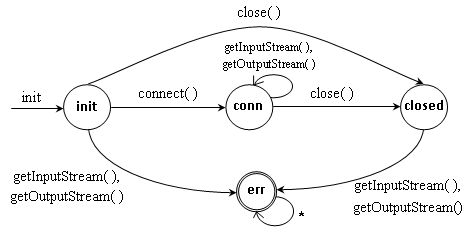
\includegraphics{./images/Fsa.png}
  \caption[FSA]{Partial typestate specification for java.net.Socket.}
  \label{fig:FSA}
\end{figure}


Figure 1.1  shows  a  finite state automaton providing a partial specification 
for the   java.net.SocketAPI. The finite state machine expresses the language of 
all program executions that violate this property. It monitors a connection's 
'close()', 'connect()' and 'getInputStream(),getOutputStream()' events and 
signals an error at its accepting state.\\\\
There are many typestate checking tools, both dynamic [4,7,8,13] and 
static[1,2,5,6], developed to ensure the correctness of property. While static 
program analysis inspect the program?Äôs code to prove the absence of typestate 
property violations for all possible executions of a given program, dynamic 
analysis tools incorporates a runtime monitor in the program under test that 
realizes the typestate properties that the program must satisfy. Testing all 
possible execution paths of complex systems endures high costs. Inorder to 
improve the
cost-effectiveness of static typestate analyses, researchers have combined 
multiple techniques [17, 18]. In [17], the authors present an intraprocedural 
analysis that eliminates the need for expensive whole-program analysis. The 
researchers have make use method annotations in the form of access permissions 
that specify typestate changes. [18] present a tool \textit{Plural} based on 
this approach and evaluate it using a few applications. Although impressive in 
many ways, these approaches still may produce false positives. Also, abnormal 
behaviour can be caused due to the deployment configurations and usage scenarios 
which cannot be examined by statically based testing techniques. \\As a result, 
dynamic analysis or runtime monitoring has gained considerable attention over 
static analysis. Researchers in runtime verification have developed powerful 
runtime monitoring tools [4,7,8,9,13]. These tools instrument the program under 
test with a runtime monitor and then, by composing the monitor with the program, 
the 
monitor observes the occurrence of each transition and decides whether the 
properties have been met or violated. Events are generated as a result of the 
instrumentation which keeps track of typestates. One important drawback of 
monitoring is that the instrumentation added to the program under test can yield 
significant overhead which hinders the monitoring of the application in 
practice. Depending on the program and property that are monitored, the overhead 
can vary significantly because the overhead depends on both the number of 
monitors that are created and the number of events generated during the program 
execution [14].\\\\
There have been several attempts earlier to optimise the runtime monitoring. 
[15, 16] present optimization techniques to reduce the overhead caused by the 
runtime overhead. They present techniques to remove unnecessary monitor 
instances. A number of hybrid techniques which combine static analysis and 
dynamic analysis to reduce the overhead have been proposed. In recent years the 
researchers[10, 12] have tried to apply the hybrid approach in which typestate 
property violation is first checked by static analysis to reduce the number of 
monitors at runtime monitoring. In [7], Arnold et al presents QVM that checks 
violations of correctness properties and has an overhead manager that enforces 
an overhead within limits. It is built on JVM so, comes with the cost of non 
portability.\\\\ 
In our research, we aim to create a framework based on sampling of objects for 
runtime monitoring that is deterministic and memory efficient. In our approach, 
we investigate the trade-off between the runtime overhead and the error 
reporting.  We are using a novel approach that works by limiting the number of 
monitors based on heuristics that are related to the program execution context. 
Depending on whether an object that is analysed has been previously monitored or 
not, the decision to sample the objects is made. In other words, monitoring will 
be performed only for the sampled objects to ensure that there is  redundancy 
among monitor's behavior of detecting the same error again and again. The total 
number of monitors generated for analysing the violations is restricted. In 
addition, the approach also limits the number of monitors that are associated 
with events related to a set of objects. Only a limited number of monitors are 
generated, thus utilizing memory efficiently. We have presented a cost model 
that aims to provide worst-case bounds for the execution times of handling 
events.\\\\
We implemented the sampled object based runtime monitoring framework on JavaMOP 
[4]. We used our framework to monitor two typestate properties, HasNext and 
UnsafeIterator, on some of the benchmarks from the Dacapo benchmark suite[11] 
and were able to capture the violations even after limiting the generation of 
monitors. We have also defined a cost model that gives the cost incurred in 
runtime monitoring by our approach to show that it is deterministic in terms of 
execution time.\\\\
\textbf{Outline} The rest of the report is as follows: Chapter 2 explains the 
motivation behind this research work. Chapter 3 provides a detailed overview of 
Sampled Object based Monitoring and shows an example. Chapter 4 presents the 
Cost Model of our approach. Chapter 5 presents our experimental data. Chapter 6 
discusses the related work. Chapter 7 provides some concluding remarks.
}

\setlength\floatsep{5pt}
\setlength\textfloatsep{5pt}
\setlength\intextsep{5pt}

\section{Background and Motivation}
\label{sec:motivation}

%% UnsafeIterator is NOT a JAVA property!

\subsection{Finite State Properties}
\label{sec:motivation:fsp}

\begin{figure}[t]
\centering
  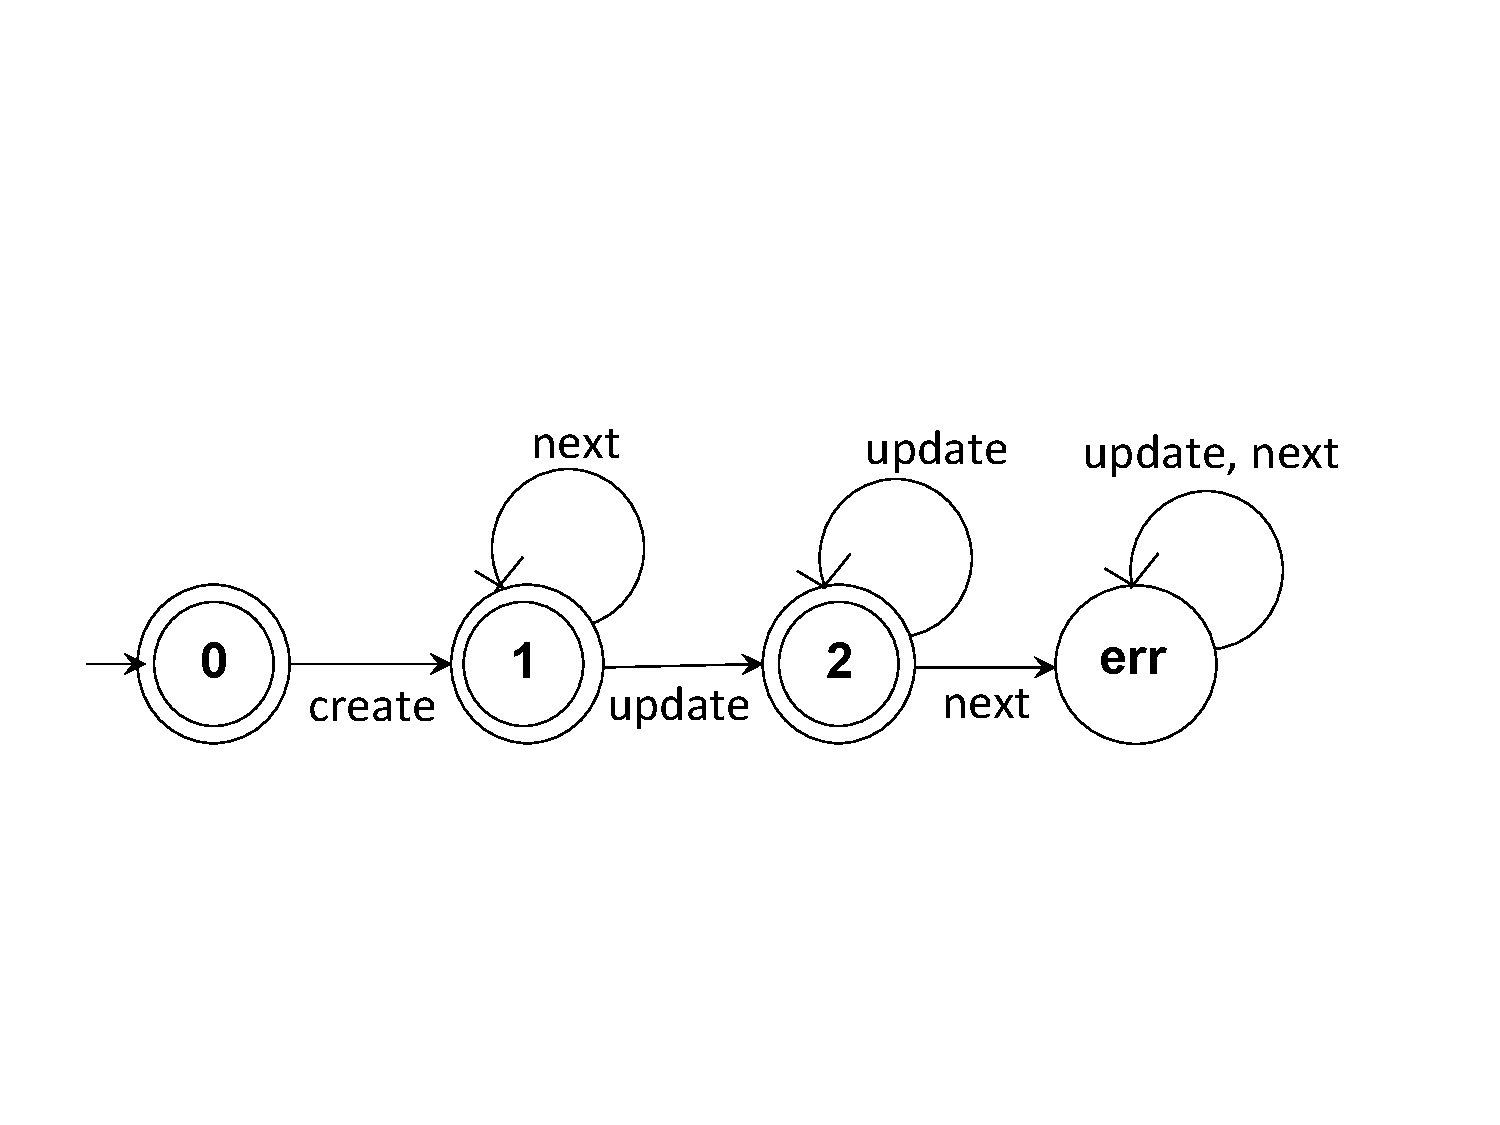
\includegraphics[scale=0.3, trim=0 5cm 0 6cm]{./images/unsafeiterator.pdf}
  \caption[UnsafeIterator Property FSA]{UnsafeIterator Property.}
  \label{fig:unsafeiteratorfsa}
\end{figure}

\begin{figure}[t]
\centering
  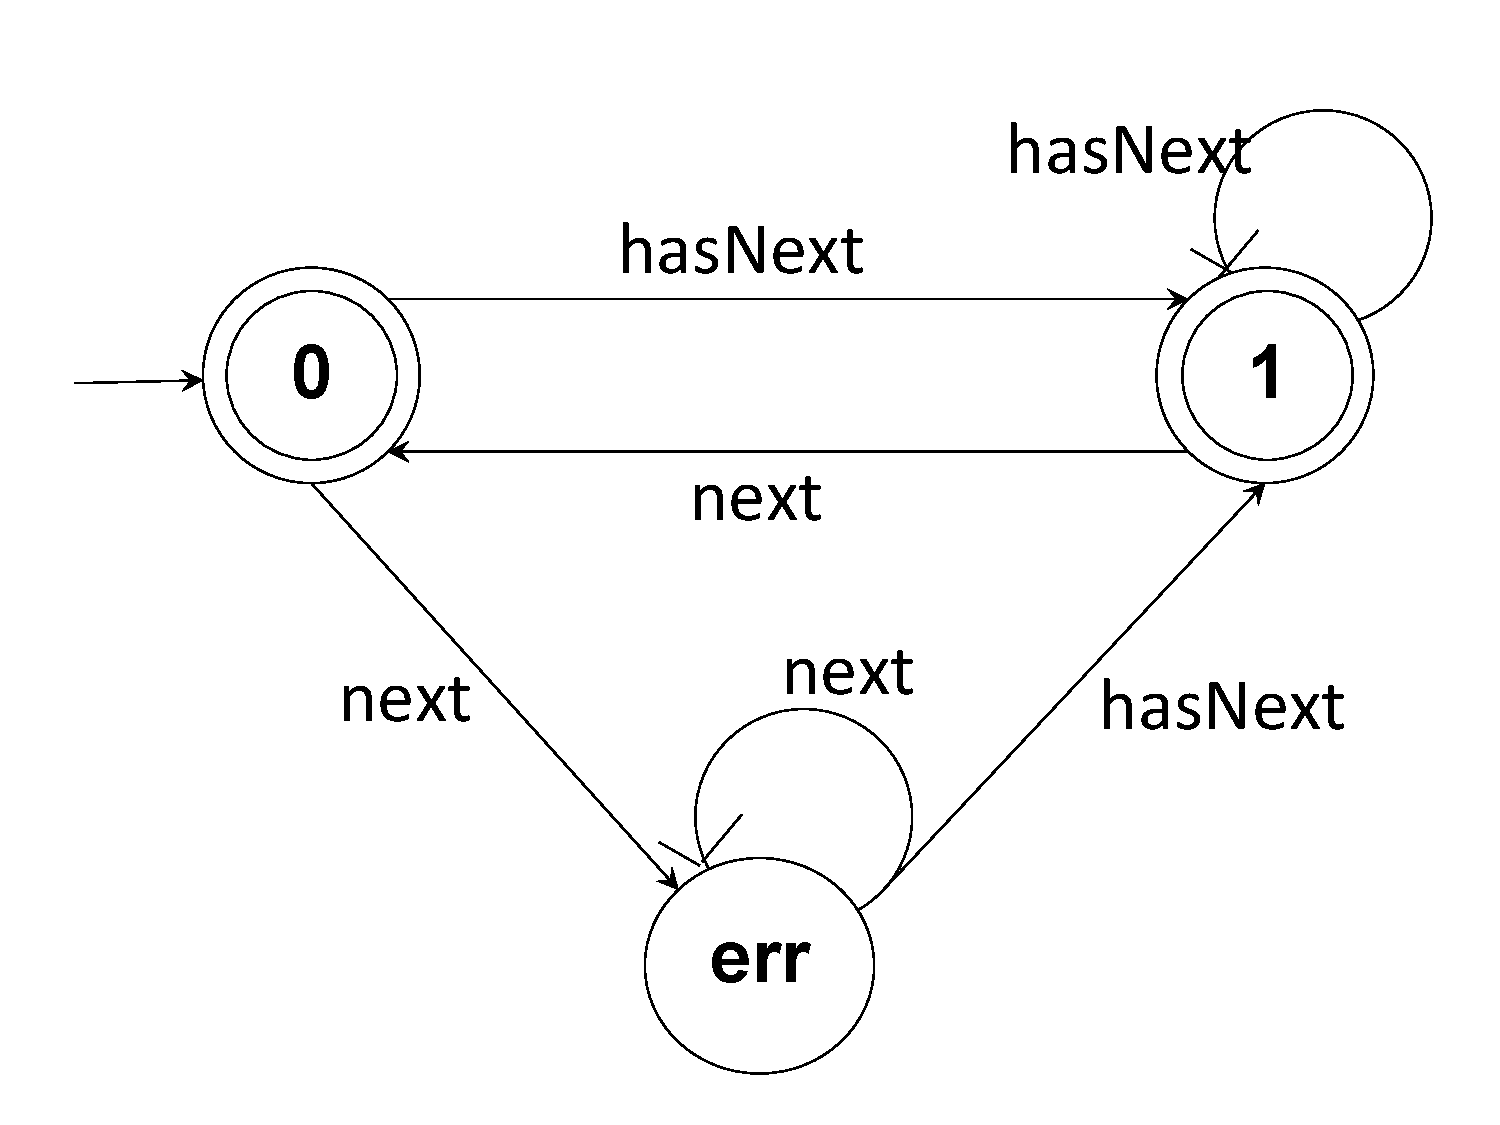
\includegraphics[trim=20cm 0cm 15cm 1cm, scale=0.2]{./images/HasNext.pdf}
  \caption[HasNext Property FSA]{HasNext Property.}
  \label{fig:hasnextfsa}
\end{figure}

Finite state properties that we consider in this work are either typestate
properties or typestate-like properties involving multiple objects that can be
modeled using a finite state automaton (FSA) \cite{Strom:TSE86}.

Figure~\ref{fig:unsafeiteratorfsa} depicts an FSA, 
which models iteration over a \code{Collection}, and codifies that a 
\code{Collection} must never be updated while it is being iterated over. The 
symbols \textit{create}, \textit{update}, and \textit{next} correspond to 
creating an \code{Iterator} from a \code{Collection}, modifying the 
\code{Collection}, and iterating over the said \code{Collection}, respectively. 
As shown in the figure, the symbol \textit{next} (observed following an 
\textit{update}) indicates iteration after a \code{Collection} update, and 
pushes the FSA to the \textit{error} state. Similarly, 
Figure~\ref{fig:hasnextfsa} encodes \code{Iterator} property \code{HasNext}, 
which states that \code{HasNext} must be invoked every time prior to invoking 
\textit{next} to ensure that the object exists before it is operated upon.

\subsection{Monitoring Systems}
\label{sec:motivation:monitor}

\begin{figure}[t]
\centering
  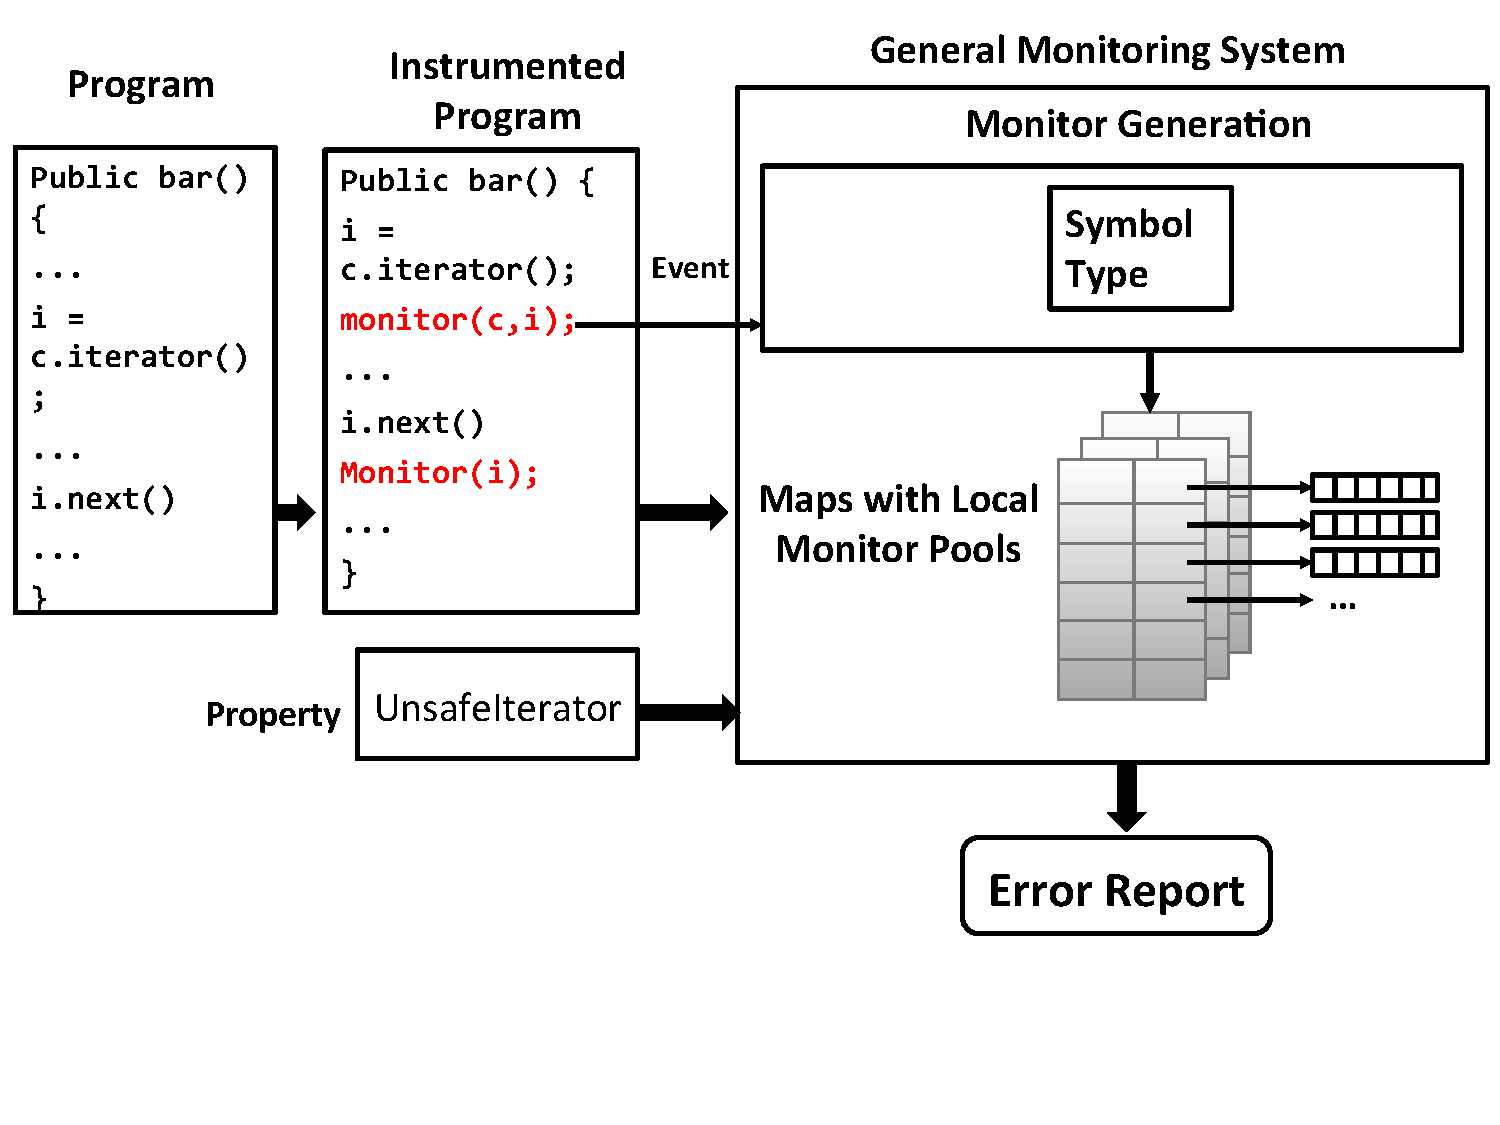
\includegraphics[width=\linewidth, trim = 0 2cm 0 0]{./images/general_monitoring_scheme.pdf}
  \caption[Schematic of Memory-efficient and Time-Deterministic Monitoring 
System]{Schematic of Memory-efficient and Time-Deterministic Monitoring System.}
  \label{fig:general_schematic}
\end{figure}

Figure~\ref{fig:general_schematic} depicts a general monitoring scheme that takes as 
an input an instrumented program and a property to be monitored. The program
instrumentation corresponds to the extra code added for program statements 
that are relevant to the property. This extra code generates events at the runtime
which are tracked by the monitoring system. An event is parameterized by
the objects and it has a symbol associated with it. This information is analyzed
by the monitor creation module to see if a new monitor needs to be created. A
monitor may contain a property FSA, references to the associated objects, and its
current state. If the system decides to create a new monitor, a monitor is created
and added to various pools
associated with the related objects, and then tracked for all future events
related to it. In case a monitor moves to the error state, it reports the error.

\code{Collection}s and \code{Iterator}s are commonly used objects, and also 
frequent sources of errors \cite{}. Thus, common monitoring systems, like 
\textsc{JavaMOP} typically instantiate a \textit{monitor} corresponding to every 
pair of \code{Collection} and \code{Iterator}, and use it to track the 
specified finite state properties upon occurrence of every event. For example, 
the monitoring system may create a new monitor for the \textit{creation} event, 
which corresponds to an invocation to the \code{Iterator()} method on the 
\code{Collection} interface, and returns an instance of the \code{Iterator}.
This newly created monitor is associated with both the \code{Collection} and 
the \code{Iterator} objects.

%% why is it a challenge
\myparagraph{Challenges} Efficient monitoring of finite state properties is 
thus usually a challenge due to:

\begin{table}[t]
\centering
\scriptsize
\begin{tabular}{|c|c|c|c|c|c|c|}
\hline
\multirow{2}{*}{} & \multicolumn{2}{c|}{HasNext} & 
\multicolumn{2}{c|}{UnsafeIterator} & \multicolumn{2}{c|}{HashSet}\\
\cline{2-7} 
                  & monitors     & events        & monitors         & events   
                  & monitors         & events \\ \hline
avrora      & $0.8$M & $1.5$M  & $0.9$M  & $1.4$M  & $106$ & $11$K \\\hline 
bloat   & $1.9$M  & $162$M & $1.9$M  & $82$M   &$66$K& $84$K  \\\hline 
pmd  & $8.6$M      & $47$M      & $1.9$M    & $26$M & $6.8$M & $3.5$M\\ \hline
chart  & $817$ & $6.8$K    &  $817$  & $568$K & - & -\\ \hline
\end{tabular}
\caption{Number of monitors created and events generated for different programs 
and properties. %\note{Get numbers for all benchmarks.}
}
\end{table}
\label{table:numofmonitors}

\begin{table}[t]
\centering
\scriptsize
\begin{tabular}{|c|c|c|c|}
\hline
%\multirow{2}{*}{} & \multicolumn{2}{c|}{HasNext} & 
% \multicolumn{2}{c|}{UnsafeIterator} \\ \cline{2-5}
 {} & Original & HasNext & UnsafeIterator\\
 \hline
avrora            & 0.1G      & 0.4G(300\%)       & 0.7G(600\%)           \\ 
\hline
bloat             & 0.5G      & 1.1G(120\%)    & 1.3G(160\%)              \\ 
\hline
pmd               & 0.5G      & 0.6G(20\%)     & 1.0G(100\%)             \\ 
\hline
\end{tabular}
\caption{Memory consumption for different programs and properties with and 
without monitoring. The figures in the parentheses are the percentage 
overheads. %\note{Get numbers for all benchmarks.}
}
\end{table}
\label{table:consumedmemory}

\begin{challenges}
 \item \textbf{High monitor count}: Typically, in practice, a \code{Collection} 
object may get iterated over several times before getting garbage collected. 
Coupled with the fact that both \code{Collection}s and \code{Iterator}s are 
frequently used objects in most programs, the number of monitors grows 
exponentially. Table~\ref{table:numofmonitors} lists the huge number of 
monitors observed when monitoring three commonly used \textsf{DaCapo} benchmarks 
for \code{HasNext} and \code{UnsafeIterator} properties using with JavaMOP 
v$2.3$. The huge number of monitors even for a relatively small number of 
monitored \code{Collection} and \code{Iterator} objects puts a significant 
burden on the system and the garbage collector. Furthermore, if the monitor 
objects are live, the garbage collector cannot even reclaim them.
 
 \item \textbf{High memory usage}: Table~\ref{table:consumedmemory} lists the 
memory consumption of the benchmarks with and without monitoring using 
\textsc{JavaMOP} v$2.3$. We observe that the large number of monitors results 
significantly large memory consumption, in contrast to the benchmarks' normal 
memory requirements, \ie\ without monitoring. Furthermore, in practice, 
programmers like to monitor programs for \textit{all} interesting properties 
collectively, and not individually. This collective monitoring of properties 
becomes extremely difficult, and often infeasible. Prior 
work~\cite{Purandare:2013} presents a technique to compact multiple 
monitors and track programs for several properties simultaneously. However, the 
resource footprint can still be significant and prohibitively high for 
resource-constrained systems, because compaction reaches its limit quickly when 
involving a finite state automata (FSA) product, which may itself grow 
exponentially.

 \item \textbf{High event tracking overhead}: In addition to the high overall 
resource consumption associated with monitors, the cost of handling individual 
events for tracking properties associated with multiple objects, such as 
\code{UnsafeIterator}, could potentially be prohibitive. This high cost is 
incurred since, theoretically, an unbounded number of monitors may get 
associated with the events (depending on the program and property interactions). 
As a result, the cost of tracking even a single event can become unpredictably 
large.
% 
In fact, we observed that over $1500$ monitors were associated with a single 
\code{Collection} object when monitoring for \code{UnsafeIterator} property 
for the \text{bloat} \textsf{DaCapo} benchmark. Since each of these monitors 
needs to be tracked when an event is handled by the corresponding receiver, 
monitoring all events, thus, becomes non-deterministic in terms of time. 
Furthermore, not being able to provide guaranteed bounds on the monitored 
execution significantly restricts the usage to non real-time systems or systems 
where performance guarantees are not essential. In any case, however, most 
systems suffer degraded performance with uncontrolled resource usage and 
execution overhead for monitoring systems.
 
 \item \textbf{Redundant monitors}: For the same set of \textsf{DaCapo} 
benchmarks and properties, we also observed that all $42$ errors reported while 
monitoring \textit{bloat} for property \texttt{HasNext}, and $333$ errors 
reported by \textit{pmd} can be partitioned into two distinct classes of errors 
that shared similar execution context, \ie\ method calls.
% 
% % we need not explain the optimization here.
% For this work, we associated an execution context with a method calling 
% sequence
% %a call stack and the program counter,
% and the data was collected  by considering limited execution context for 
% efficiency reasons. 
% 
These observations indicate that several monitors catch the same redundant 
errors, which clearly is not intelligent reporting to the developer. Ideally, 
the monitors must report only distinct errors, \ie\ only $3$ distinct errors 
for \textit{bloat}, and $2$ for \textit{pmd}. 
%\note{This needs to be clarified --- 2 distinct classes, and 3 and 2 errors respectively.}
Hence, we believe that sampling-based monitoring that leverage the program execution 
context would be significantly more effective and consume much less resources.
\end{challenges}

%We also made some fine-grain observations regarding the redundancy in the 
%behavior of monitors.  For the same DaCapo benchmarks and properties, 
%Table~\ref{table:joinpoints} presents the number of \textit{observable} 
%statements that generate monitoring events. Even though monitors are generated 
%in millions, observable statements are only a few. This indicates that there 
% is 
%a reason to believe that the \textit{programming contexts} under which these 
%statements are invoked are limited. 

In this work, we present a runtime verification approach that exploits 
redundancy in monitor behavior, and retains only those that show distinct 
behavior. As a result, put approach significantly improves upon memory 
efficiency and execution time determinism. 
% The approach has been described in detail in Section~\ref{sec:approach}.

\ignore{
Figure~\ref{fig:unsafeiteratorfsa} depicts a finite state automaton (FSA) that 
models a property \texttt{UnsafeIterator} which is defined by the API of Java 
standard library and is related to a \texttt{Collection} as well as an 
\texttt{Iterator} object. It specifies the rule that a collection should not be 
updated while it is being iterated. The symbols \textit{create}, 
\textit{update}, and \textit{next} correspond to creating an iterator from a 
collection, modifying a collection, and iterating over a collection 
respectively. Hence, as shown in the figure, the symbol \textit{next} observed 
after the symbol \textit{update} would indicate iteration after a collection 
update which pushes the FSA to the \textit{error} state. Monitoring systems 
typically instantiate a monitor corresponding to every such pair of a collection 
and an iterator and use it to track the FSA states depending on the sequence of 
operations or events encountered.

In practice, a collection object may get iterated several times in its life 
time. On the occurrence of a \textit{creation} event, that may correspond to the 
call to \textmd{Iterator()} method in the \textmd{Collection} interface that 
returns an iterator, a monitoring system may create a new monitor for tracking. 
The newly created monitor is associated with the collection object and also the 
iterator object. It is easy to see that since the collection and iterator are 
frequently used objects in many programs the number of monitors may grow 
quickly. This puts heavy burden on the system and the garbage collector. 
Moreover, if the monitor objects are live, garbage collector cannot reclaim 
them.

Similar issue arises with another iterator property \texttt{HasNext} depicted in 
Figure~\ref{fig:hasnextfsa}. It specifies that a call to the \textit{hasNext} 
method must be given before calling \textit{next} method to ensure that an object 
exists before it is used. Collections and iterators are not only commonly used 
objects, but often the sources of error \cite{}.
}

\ignore{
Monitoring finite state properties efficiently has been a challenge due to the 
large number of monitors that may get created and also due to the large number 
of monitors that may get associated with some events. 
Table~\ref{table:numofmonitors} shows the number of monitors we observed while 
monitoring some \textsf{DaCapo} benchmarks using JavaMOP 2.3 for 
\texttt{HasNext} and 
\texttt{UnsafeIterator} properties.
}

\ignore{
\begin{itemize}
\item {\bf HasNext}: Every call to method \texttt{next} associated with an 
iterator must be preceded by a call to method \texttt{hasNext}.
\item {\bf UnsafeIterator}: A collection should not be updated while it is being 
iterated.
\end{itemize}
}

\ignore{
Table~\ref{table:consumedmemory} presents the memory consumption of the 
benchmarks with and without monitoring when JavaMOP 2.3 was used for monitoring. 
It shows that the large number of monitors results in the consumption of 
significantly large amount of memory in comparison with the benchmarks' memory 
requirements. Moreover, in practice, programmers would like to monitor their 
programs for all of the interesting properties together, not separately. This 
only means that runtime monitoring would become extremely difficult or even 
infeasible when properties are monitored simultaneously. Purandare et al. 
present a technique that compacts several monitors into one and tracks programs 
for multiple properties simultaneously \cite{}. However, even though the compaction 
reduces the footprint of a monitored program to a certain extent, the footprint 
can still be significant and prohibitively high for 
resource-constrained systems. This is owing to the fact that the compaction 
reaches its limit quickly since 
it involves taking a finite state automata (FSA) product which may grow 
exponentially.
}

\ignore{
In addition to the overall high overheads, for the properties associated with 
multiple objects, such as \texttt{UnsafeIterator} the cost of handling 
individual events can also be very high. This  happens since theoretically unbounded number of 
monitors may get associated with the events depending on the program and 
property interactions. As a result, the cost of tracking one single event can become 
unpredictably large. In fact, it was observed while monitoring for 
\texttt{UnsafeIterator} property for the \textsf{DaCapo} benchmark 
\textit{bloat} that as many as 1548 monitors had got associated with a single 
\textsf{Collection} object. Each of these monitors needs to be tracked when an 
event is seen by the corresponding receiver object. As a result, monitoring 
actions become nondeterministic in terms of time. Not being able to provide
bounds to the monitoring execution can 
restrict the usage of monitoring to nonreal-time systems or systems where 
performance guarantees are not essential. 
However, most systems in practice would suffer due to degraded performance if 
the memory overheads and execution times of monitoring cannot be controlled.

%We also made some fine-grain observations regarding the redundancy in the 
%behavior of monitors.  For the same DaCapo benchmarks and properties, 
%Table~\ref{table:joinpoints} presents the number of \textit{observable} 
%statements that generate monitoring events. Even though monitors are generated 
%in millions, observable statements are only a few. This indicates that there is 
%a reason to believe that the \textit{programming contexts} under which these 
%statements are invoked are limited. 

For the same \textsf{DaCapo} benchmarks and properties, we made some fine-grain 
observations regarding the redundancy in the behavior of monitors. We observed 
that the 42 errors reported while monitoring \textit{bloat}  for property 
\texttt{HasNext} could be partitioned into two classes of errors such that all 
errors in a class had a similar \textit{execution context}. Similarly, we could 
divide 333 errors reported by \textit{pmd} into two classes. For this work, we 
associated an execution context with a method calling sequence
%a call stack and the program counter,
and the data was collected  by considering limited execution context for efficiency 
reasons. These observations indicate that many monitors catch redundant errors, 
which are not so useful to developers. Ideally, the reporting should only be 
performed for distinct errors which means catching only thee distinct errors for 
\textit{bloat} and two for \textit{pmd} would suffice. Hence, we believe that 
monitoring performed by sampling objects based on the program execution context 
could be effective and would require less resources. 

In this work, we present a runtime verification approach that tries to exploit 
the redundancy in the monitor behavior and retain only the ones that show 
distinct behavior. As a result, it improves on memory efficiency as well as execution time 
determinism. The approach has been described in detail in 
Section~\ref{sec:approach}.
}

\ignore{
Some very particular typestate properties are typically desired to be satisfied 
by all programs. The traditional runtime-verification approach has been 
developed over the past decade to analyze large complex applications because of 
several desirable properties. For instance, because the monitor specifications 
can be very expressive as runtime monitoring reason about concrete program 
events and runtime objects, and thus avoid false warnings. Also, when a runtime 
monitor detects a property violation, it can respond to this violation in many 
different ways, which can be any code from information logging to runtime 
recovery. The programmer has the guarantee that the monitor will detect a 
violation if it exists.\\
\begin{table}[h]
\centering
\begin{tabular}{|c|c|c|c|c|}
\hline
\multirow{2}{*}{} & \multicolumn{2}{c|}{HasNext} & 
\multicolumn{2}{c|}{UnsafeIterator} \\ \cline{2-5} 
                  & monitors     & events        & monitors         & events     
      \\ \hline
avrora            & 805500       & 1507792       & 909011           & 1365801    
      \\ \hline
bloat             & 1906736      & 162227791     & 1876472          & 82032703   
      \\ \hline
pmd               & 8576900      & 47231567      & 1949816          & 25958426   
      \\ \hline
\end{tabular}
\caption{Number of monitors created and events generated for different programs 
and properties}
\end{table}

On the other hand, existing tools for runtime monitoring usually incur an 
unacceptable overhead. Large number of monitors created during runtime and the 
events generated by the program execution are responsible for the overhead. In 
our experiments, for Dacapo benchmarks bloat and pmd benchmarks create nearly 
the same number of monitors, in excess of a few million, for property 
UnSafeIterator for JavaMOP[4]. Table 2.1 shows the large number of monitors 
created and the events generated during runtime of several programs from Dacapo 
Benchmark suite.
\\\\With the motivation that there is a large redundancy among monitors in terms 
of their behavior which results in many monitors detecting same errors, we 
investigate the trade-off between the runtime overhead and the error reporting. 
We propose a runtime verification framework that is memory efficient and time 
deterministic and can be used for real time embedded systems. The framework has 
the following characteristics:
\begin{itemize}
	\item \textit{Object based sampling}: we introduce object based sampling 
to collect sampled objects on which monitoring will be performed. The heuristics 
applied for sampling are related to the program execution context. We achieve it 
by obtaining the call-stack contents.  obtain the method calls invoked on the 
current runtime object under analysis and compare whether the trace of method 
calls of that object has been previously seen during runtime. 
	\item \textit{Deterministic monitoring}: For multi-object properties 
such as UnsafeIterator property, an event such as update can get associated with 
several monitors. This number can grow uncontrollably and can be as large as 
1548 for an event [9]. It becomes difficult to keep track of every monitor for 
that event. Hence, the whole operation of handling events may become non 
deterministic as far as timing requirements are concerned. We consider a 
monitoring behaviour to be deterministic as we can calculate the time taken to 
perform monitoring by the cost model presented. We are controlling the monitors 
associated with each event to make tracking deterministic.
	\item \textit{Limited number of monitors to make memory efficient}: we 
consider to limit the total number of monitors generated while runtime 
verification and at the same time maintaining sufficient accuracy for detecting 
property violations.
\end{itemize}
Runtime Monitoring is complete but fundamentally unsound since it cannot see 
anything beyond the current execution. In our approach, we sacrifice on the 
soundness to achieve memory efficiency and determinism in terms of time.
}
\section{Monitoring Approach}
\label{sec:approach}

Our optimized monitoring approach strives to reduce the memory requirements
of finite state monitoring and make it efficient. At the same time it also tries to make monitoring more 
time-deterministic without compromising too much with its error reporting. The following subsections
give an overview of the approach, and describe the monitoring algorithm as well as its key features.

%The approach is based on the following mechanisms.

%Section~\ref{subsec:outline} gives the outline of our approach, and
%Section~\ref{subsec:algo} presents the algorithm.

\subsection{Outline of the approach}
\label{subsec:outline}

\begin{figure}[t]
\centering
  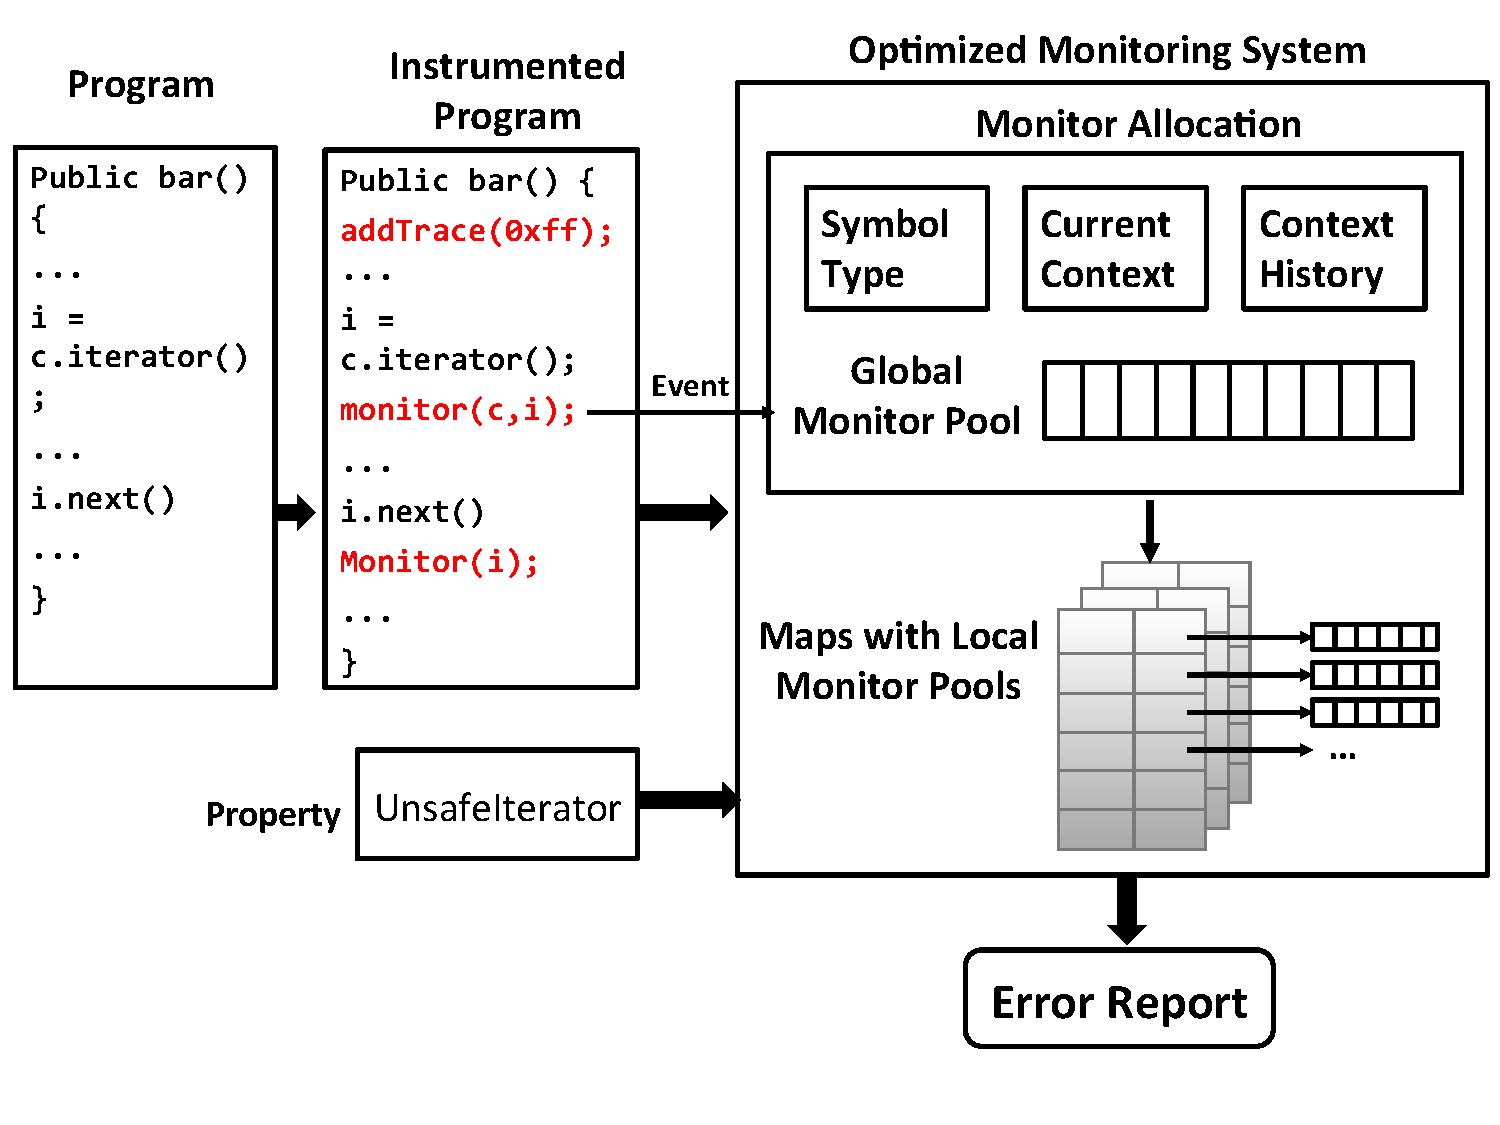
\includegraphics[width=\linewidth]{./images/optimized_monitoring_scheme.pdf}
  \caption[Schematic of Memory-efficient and Time-Deterministic Monitoring 
System]{Schematic of Memory-efficient and Time-Deterministic Monitoring System.}
  \label{fig:schematic}
\end{figure}

Figure~\ref{fig:schematic} shows the main elements of our approach. The program 
under execution generates events parameterized by objects which are accepted by 
our monitoring system, and each one of them is handed over to the monitor 
allocation module. This module contains information about the symbol types, the current execution context, 
the history of the observed execution contexts, and the global monitor pool.
Based on the type of the symbol, which is part of the event, and some heuristics 
based on the program execution context, the allocation module makes a decision about whether to allocate a monitor or not.
For convenience, if not already available, we 
specify explicitly the program points that generate creation events, so that the 
approach can leverage this information to make a decision about monitor allocation and tracking. 
If the event is of creation type, the allocation module checks the execution context and its 
tracking history to see if the context was already seen in the past, and if yes, 
then with what frequency. The system probabilistically skips the monitor 
allocation phase for frequently seen contexts. The contexts can generally be maintained as
trees in which case a new context either adds a new branch or new branches and a leaf node. 
Every leaf node uniquely defines a context and it keeps information about the 
number of times the context was seen. Currently, the seen contexts are stored as bitmaps to enable efficient
comparisons, and this mechanism can be improved further for efficiency.

The global monitor pool is implemented as a circular array that preserves 
the chronological ordering. In case the allocation module chooses to allocate a monitor,
it picks the next available monitor for allocation. The monitor being allocated could be already in use.
In this case the monitor is first removed from the existing local pools of the associated 
objects, and then reallocated to the new objects under consideration. This allocation results in the monitor
getting added to the local pools that belong to the associated objects. The local pools also have a limit of their mximum size.
In case, any of the concerned local pool is already full, the oldest monitor from the pool is removed and returned to the global pool
to create room for the new monitor. 

The tracking of monitors for the non-creation events is similar to the 
conventional monitoring system. The only difference is that if no monitor exists in the maps 
corresponding to the objects associated with the incurred event, then monitoring is completely 
skipped for that event. This case can only happen when the monitors corresponding to the 
associated objects were intentionally not created by the system. Skipping monitoring events is a 
direct saving in terms of execution time overhead. In case any of the monitors goes to the error state,
an error report is generated.


\subsection{Context-based sampling}

We use context-based sampling of objects to control the 
number of monitors. The motivation for this approach comes from our observation 
that monitors created at the same creation site and under similar program
execution context tend to go through a similar life cycle. In other words, these monitors are more 
likely to show a redundant behavior. Hence, the heuristic applied for this 
sampling is based on the program execution context. Our approach works by i) identifying 
the monitor creation sites which are specified as creation events in the 
monitoring specification, and then by ii) obtaining the method calling sequence to identify 
the execution context, and finally by iii) making a decision about the 
allocation of the monitor based on the number of times this context was seen in 
the past. More often the monitoring system has seen the context, less likely it 
is to allocate a monitor. The program execution context that we consider in this work is
the method calling sequence of limited length. We describe the implementation details
in Section~\ref{sec:implementation}.

\subsection{Fixed-size global pool of monitors}

We limit the total number of monitors that our monitoring approach might generate by creating a 
monitor-pool of fixed size prior to the program execution and then maintaining 
it during the execution. In short our approach reuse monitors. The monitors 
after their usage can be returned back to the system. Moreover, if the pool runs 
out of monitors and the system needs a new monitor, one of the monitors currently being 
used is forcefully reclaimed and made available for the reallocation. The 
heuristic that we use to reclaim a monitor is based on our observations that the 
program events related to the same objects are often temporally separated from the rest,
and events are more likely to be generated by newly created objects. In other words, in an execution 
trace, events related to the same or related objects often occur together.
We exploit this observation by making the oldest
monitor available for reallocation. This also means that the objects associated with that monitor
are not tracked further, and if they had observed a sequence of events that might have otherwise
lead the monitor to the error state, the approach will now miss the error. 
Potentially missing a few errors is a cost of our optimized monitoring approach.
However, by using the heuristics presented in this Section the approach tries to
minimize \textit{false negatives}. As described in Section~\ref{sec:definition}, our
goal is to detect all non-redundant errors, and not all errors.

\subsection{Fixed-size local pool of monitors for indexed objects}

In the case of properties related to multiple objects, 
an object can get associated with numerous monitors in its life-time. For example,
in the case of \texttt{UnsafeIterator} property a collection object may get associated
with numerous iterator objects in its life-time. In other words, every pair of a collection and its related
iterator has an associated monitor. Hence, a collection may have several monitors associated with it
and they are stored in a map corresponding to the collection object as a key.
Therefore, an event related to the collection object results in the states of 
several monitors getting updated. Hence, handling such events may become 
\textit{nondeterministic} in terms of their execution times even when the events are related
to a same symbol, or to a same set of objects but at different times.

For this work, we consider a monitoring behavior to be time-deterministic if we 
can compute the 
worst-case time taken to execute every monitoring event. Binding the number of 
monitors associated with an object allows us to limit the worst case execution 
time for any monitoring operation associated with that object. Our approach 
implements this constraint by allocating a fixed-size local pool of monitors to 
individual objects. We reallocate an existing monitor in case this buffer is full and we need a new
monitor for the same set of objects.



\begin{algorithm}[t]
                      % enter the algorithm environment
\caption[Algorithm]{Context-Aware Monitoring. Input: $\phi$ = 
($Q$,$\Sigma$,$\delta$,$q_{0}$,$F$, err), $\eta=(\beta, \sigma)$ where $\eta$ is an event and $\beta \in 2^O$ 
be the set of associated objects and $\sigma \in \Sigma$}          % give the algorithm 
% a caption
\label{alg1}                           % and a label for \ref{} commands later 
% in the document
\begin{algorithmic}[1]                  
   \STATE \textbf{let} $\Sigma_{c} \in \Sigma$ be the set of creation symbols
   \STATE \textbf{let} \textit{A} be the global circular array of monitors
    \STATE \textbf{let} $\psi$ : $2^O \nrightarrow 2^M$ be a mapping that returns the monitors associated with a given set of objects.
   \STATE \textbf{let} $\tau$ : $M \nrightarrow 2^O$ be a mapping that returns the objects associated with a monitor
   \STATE \textbf{let} $\pi \in \Pi$ be a finite sequence of method structures
   \STATE \textbf{let} $\zeta$ be the data structure holding program execution contexts
  
   
    \IF{$\sigma \in \Sigma_{c}$}
        \STATE $\pi$  $\leftarrow$ getExecutionContextInfo()
        \IF{isPresent($\pi$, $\zeta$) = TRUE}
           \STATE $k$ $\leftarrow$ threshold($\pi$, $\zeta$)
        \ELSE
        	   \STATE $k \leftarrow 1$
        \ENDIF
        \STATE updateExecutionContext($\pi$, $\zeta$)
        \IF{Random() $\leq k$}  
            	\STATE $m$ $\leftarrow$ $A$.nextMonitor()
        		\FORALL {$\alpha' \subseteq$ $\tau$($m$)} 
		\STATE $\psi$($\alpha'$) $\leftarrow  \psi(\alpha') / \{m\}$
        		\ENDFOR
        		\FORALL {$\alpha' \subseteq \beta $} 
			\IF{$\psi$($\alpha'$).size() = \textit{max\_mon}}
				 \STATE $m' \leftarrow$ $\psi$($\alpha'$).first();
			  	\FORALL{$\alpha'' \subseteq$ $\tau$($m'$)} 
					\STATE $\psi$($\alpha''$) $\leftarrow$  
$\psi$($\alpha''$) / \{$m'$\}
        				\ENDFOR
			\ENDIF
                		 \STATE $\psi$($\alpha'$) $\leftarrow$  
$\psi$($\alpha'$) $\cup$ \{$m$\}
        		\ENDFOR
        \ENDIF
 \ENDIF
 \FORALL{$m$ $\in$ $\psi$($\beta$)}
     \STATE $m$.cur $\leftarrow$ $\delta$($m$.cur,$\sigma$)
     \IF{$m$.cur = err}
        \STATE report$\hspace{5pt}\textbf{error}$
     \ENDIF
 \ENDFOR
 
\end{algorithmic}

\end{algorithm}
\label{algo:monitoring}



\section{Monitoring Algorithm}
\label{sec:algo}

Algorithm~1 depicts the steps that implement our monitoring scheme. It takes a
property $\phi$ and an event $\eta as input. $ Lines 7--30 
describe the operations that are performed when a creation event is encountered 
and a new monitor may need to be allocated. Line 8 reads the program execution 
context. If the execution context is already seen which is checked at line 9, 
then a \textit{threshold} value is generated based on the number of times the 
context is seen in the past; else if the context is unseen, the threshold is 
assigned the highest possible value which is 1. In either case line 14 updates 
the execution context history.
%In our implementation it involves either adding 
%new branches in the context tree if the context was unseen or only incrementing 
%the frequency count filed of the leaf node corresponding to the known context.

Lines 15--29 describe the steps when the threshold value is found to be large 
enough to justify allocation of a monitor which is checked by the condition at 
line 15. As a result, a new monitor from the global circular array is allocated
at line 16. Lines 17--19 describe the steps to reclaim the monitor in case it is previously 
assigned. This step ensures that all previous bindings are removed and the 
monitor is ready for the new assignment.

Lines 20--28 describe the steps that ensure that the local monitor pool limit is 
not reached. In case it is, the oldest monitor in the pool is reclaimed first by 
removing it from all the lists of associated objects' maps before the new monitor 
is added in the lists as shown by line 27.

Finally, as shown in lines 31--36, the relevant monitors are retrieved and their 
states are updated. In case any of the state is the \textit{error} state, then 
the error is reported. This final step is similar to the conventional 
monitoring, except that no monitor will be tracked if the system does not see 
any monitor allocated.

\subsection{Correctness}
\label{subsec:correctness}

We define correctness of our algorithm by arguing about its \textit{soundness} and \textit{completeness}
with respect to the general unoptimized approach. The major difference between 
the two approaches is in the way the monitors are generated. The unoptimized approach
creates new monitors after every creation event, whereas we either allocate them
from the pool or skip the allocation completely. The allocation can be further divided
into two cases: a) In the case when we allocate a fresh monitor from the pool, there is no
difference in the way the newly allocated monitor is tracked in the two approaches, and the
correctness argument should automatically hold. b) In the case when
we reuse a monitor, we first remove all of the current bindings by removing
the monitor from all of the local pools. This ensures that there is no undesirable side-effect
and the newly allocated monitor tracks the only events that are related to the new set of
objects. As a result \textit{false positives} are never produced and the completeness is
never compromised. Similarly for completely skipped monitors false error reports are 
never reported for obvious reasons.

Runtime monitoring is inherently 
unsound \cite{}. It can report only based on what it has observed. This means errors 
may not be reported if the paths that encounter them are not exercised. In both of the allocation cases
discussed above, if the newly allocated monitor gets reallocated in the future before it can report
any error, we may lose the system's soundness further with respect to the unoptimized approach. The same argument 
applies to the skip case. Note that all monitors apart from the one that gets reallocated continue
their functioning in a way similar to the unoptimized monitoring, and report errors as and when they detect any.

\subsection{Memory and Time Efficiency }
\label{subsec:memory efficiency}

The algorithm preallocates monitors from a pool of constant size, and then if 
required, monitors are reused. In our study we varied the pool size from 1k 
to 30k monitors. This results in the reduction of the number of required monitors 
considerably especially for challenging program and property combinations in 
which a very large number of monitors may get generated. In fact, as the study indicates,
for some configurations the system ended up consuming
even less monitors than the size of the global monitor pool due to
limited program execution contexts that were
observed during runtime. This shows that an approach based on the execution
contexts may result in a dramatic saving in the memory requirements of a
software application.

The reduced number of monitors allow us to skip monitoring actions. Even though
maintaining and checking execution contexts as well as reclaiming monitors add to the overhead, 
a simple memory management that involves easy monitor allocation from fixed-size pools helps maintain the
system's efficiency. In addition, it reduces the system's dependence on the garbage collector since no
monitors need to be cleaned. Apart from saving execution time it also reduces the unpredictability
of the execution time introduced by the garbage collector.

\subsection{Time-Determinism}
\label{subsec:timedeterminism}

It is easy to see that the algorithm has fairly tight worst-case execution time bounds
for all of its steps making it time-deterministic. This can be explained
by analysing the bounds on the steps involved in handling a monitoring event.
We divide the event-handling analysis into the following two categories.

\paragraph{Handling of creation events} A creation event may result in a monitor
allocation depending on the program execution context under which it was generated.
Accessing the context on line 8 is a constant time operation. Method \code{isPresent} on
line 9 traverses entire depth of the context tree in the worst case, which makes it
constant time since the tree has a limited height. Updating the execution context on line 14
cannot take longer than the time required to traverse the depth of the tree for the same reason.
The loop on lines 17--19 iterates $2^n$ times and hence takes $O(2^n)$ time 
where $n$ is $\mid\tau(m)\mid$ and $\tau(m)$ is the number of associated objects 
and is normally less than four. Hence, this operation takes $\Theta(1)$ time. By the same arguments
loops on lines 23--25 and 20--28 iterate $2^{\mid\tau(m)\mid}$ and $2^\beta$ times and take $\Theta(1)$
time since these numbers are small and often less than four. Hence, the worst case running time
of the outer loop on lines 20--28 is $\Theta(1)$. Therefore the time taken by a creation event in the
worst case is constant.

\paragraph{Handling of other events}
Since the size of the local monitor pools is limited to a small number, the loop on lines 31--36
executes at most $k$ times where $k$ the size of the local monitor pool. For properties, that are
associated with only one object this number is one. Hence, the handling of other events takes a
constant time irrespective of the objects associated with the property.

Hence, we see that the algorithm has worst case execution time of
$\Theta$(1). For a program execution that  generates $n$ events, the time taken to handle 
these events by our approach in the worst case is $O(n)$. In comparison, in the worst case,
the unoptimized algorithm may create $O(n)$ monitors, assign all of them to a set of objects,
 and then receive events of similar kind on the same set of objects
 requiring all of the created monitors to be tracked for every event. Therefore, the worst-case complexity of the
 unoptimized algorithm where $n$ is the number of events would be $O(n^2)$. Even though we expect this worst case to arise 
 in the practice rarely, we expect our algorithm to work faster than the unoptimized algorithm in the practice.
 
\subsection{Soundness, Memory, Efficiency, and Time-Determinism: Tradeoffs}
\label{subsec:tradeoff}

There is unfortunately a tradeoff between soundness of the system and the
number of monitors allocated, which in turn, corresponds to the memory allocated
for monitoring, and we pick one at a potential loss of the other.
%However, runtime monitoring is inherently 
%unsound \cite{}. It can report only based on what it has observed. This means errors 
%may not be reported if the paths that encounter them are not exercised.
We stretch the inherent unsoundness of any monitoring system a little bit further to achieve substantial benefits in 
terms of memory savings, and at the same time use heuristics that help maintain
the system's soundness.  As a result, our technique should enable developers to employ runtime 
monitoring in resource-constrained system settings where the previous 
techniques for finite-state monitoring might not have been feasible.

Similar tradeoffs exist between soundness and efficiency, and soundness and time-determinism.
However, binding worst-case execution times has its own merits 
especially in the domain of real-time systems or with systems requiring high performance.
Hence, our approach uses effective heuristics based on our observations and experience so as to reduce false 
negatives and improve the soundness of the system. As indicated by the study
in Section~\ref{sec:evaluation}, the approach can save considerable amount of
memory, improve its efficiency, and can also make monitoring time-deterministic.

Since, the monitors that produce errors are continuously tracked from the beginning similar to the
conventional unoptimized approach, the optimized approach does not 
compromise with its \textit{completeness} , and ensures that no false positives 
are ever produced.


\ignore{
\subsection{Memory-Efficiency and Time-Determinism}
\label{subsec:efficiencyanddeterminism}

The algorithm preallocates monitors from a pool of constant size, and then if 
required, the monitors are reused. In our study we varied the pool size from 1k 
to 30k monitors. This results in reducing the number of required monitors 
considerably especially for challenging program and property combinations in 
which a very large number of monitors get generated. As our study indicates, our approach 
may result in a dramatic saving in the memory requirements of a software.

It is easy to see that the algorithm has worst-case time bounds for all of its 
steps making the algorithm time-deterministic. Fetching current execution 
context in the form of a call stack is an expensive but still a constant time 
operation. The execution context tree has a bounded depth which we have limited 
to four in our prototype implementation. Hence performing read or write 
operations on it as in lines 11 and 16 are time-bound operations.

Depending on the map implementations, all the map operations such as the ones on 
lines 20, 26, and 29 are constant-time operations. The \textit{for} loops on 
lines 19, 22 and 25 iterate only a small finite number of times depending on the 
number of objects involved in the event which is typically either one or two. 
The \textit{for} loop on line 33 executes at most \texttt{MAX\_MON} times since 
that is the limit on the size of local monitor pools associated with objects.

We show in Section~\ref{subsec:tradeoff} that the algorithm has worst case bound of
$\Theta$(1). In which case the worst-case complexity of this algorithm is $O(n)$
where $n$ is the number events encountered. In comparison, in the worst case,
the unoptimized algorithm may create $O(n)$ monitors, assign all of them to a set of objects,
 and then receive events of similar kind on the same set objects
 requiring all of the created monitors to be tracked together.  The complexity of the
 unoptimized algorithm then would be quadratic. Even though we expect the worst case to arise 
 in the practice rarely, we expect our algorithm to work faster than the unoptimized one in the practice.
 }








\ignore{
\section{Simple Code and Property Example:}
While JavaMOP represents state of art runtime monitoring, our goal is to limit 
the number of monitors associated with a set of objects. It typically models 
sequencing properties as finite state automata (FSA) and check whether a program 
satisfies them during runtime.  JavaMOP uses object based monitoring in which a 
monitor for a FSA property is a relation between a set of related objects 
created during program execution and a state of the FSA.  The execution of 
sequence of program statements (under test), related to both property and the 
set of related objects, corresponds to the sequence of FSA transitions.\\
\begin{figure}[h]
\centering
  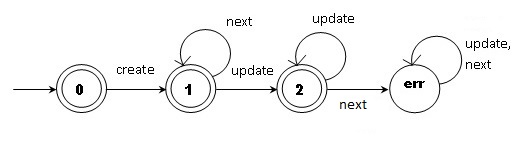
\includegraphics[scale=0.6]{./images/Unsafe.jpg}
  \caption[UnsafeIterator Property FSA]{UnSafeIterator Property.}
  \label{fig:typestateProperty FSA}
\end{figure}
\\Let us assume we are monitoring UnsafeIterator property that says not to 
modify an object of class Collection while iterating over this collection at the 
same time. In this case, it would be unclear whether the program should iterate 
over the original contents or the modified contents of the collection. While 
iterating over a collection, the runtime monitoring ensures that the program 
behaviour is well-defined. In other words, the monitor checks that there should 
not be a call to any method that is updating the collection after an iterator is 
created and before an element is accessed by a call to method next. The regular 
expression for the property is (create ; next* ; update*) and Fig 3.1 shows the 
finite state automata for UnsafeIterator property.\\\\
Below shows a code snippet for a test program. The relevant statements for the 
above property are calls to methods iterator(), add(), and next() on appropriate 
receiver objects. The relevant statements in the fragment of code being 
monitored are instrumented with extra code i.e., the OBSERVE... calls to perform 
monitoring.\\\\
When the call to method iterator() is encountered, a monitoring event create is 
generated. The instrumented code maintains a map, keyed by set of related 
objects that have been involved in previous events. The values corresponding to 
the keys are the set of monitors that are associated with the objects. On 
handling the create event, if it is found that no monitors are associated with 
the collection \textit{m1} and iterator \textit{itr}, our approach will list the 
history of method calls on the object \textit{itr} (bar(a1,a2), third(a1,a2), 
second(a1,a2), first(a1,a2), main() from our example). It will analyse if there 
exists same method calls of previously monitored objects and will sample the 
object for monitoring if match is not found and it will store the history of 
method calls for this object. However, on finding a match, the object may or may 
not be considered for monitoring depending upon how frequently it has been 
monitored previously.
\begin{center}
\textbf{A code snippet}
\begin{lstlisting}

void main(String[] args) {
	  ArrayList a1 = new ArrayList();
     al.add("C");
	  al.add("A");
	  al.add("B"); 
	  ArrayList a2 = new ArrayList ();
	  first(a1,a2);
	}
void first(ArrayList a1, ArrayList a2) { 
	  second(a1,a2); 
	} 
void second(ArrayList a1, ArrayList a2) {
	  third(a1,a2); 
	} 
void third(ArrayList a1, ArrayList a2) {
	  bar(a1,a2); 
	}
void bar(ArrayList m1,Arraylist m2) {
	  Iterator itr = m1.iterator();
		   OBSERVE.create(m1,itr);
	  m2.add(?ÄúX?Äù);
		   OBSERVE.update(m2);
     while(itr.hasNext()) {
	    Object element = itr.next();
		   OBSERVE.next(itr);
	  }
	}
    
\end{lstlisting}
\end{center}


Whenever an object is sampled for monitoring, the total number of monitors 
analysing the property are checked. If the number is below the specified limit, 
a new monitor is created and references to it are associated with the new keys 
\textit{m1} and \textit{itr} and on the other hand, if the number exceeds the 
limit, the previously generated monitor is reassigned for the current objects by 
changing the references. Thus, a limited set of monitors is used for analysing 
the property violations as done in runtime monitoring. 
}














\ignore{
\begin{algorithm}[h]
                      % enter the algorithm environment
\caption[Algorithm]{Monitoring Algorithm. $\phi$ = 
(Q,$\Sigma$,$\delta$,$q_{0}$,F), e=(l,b) where e is an event and l $\in \Sigma$ 
and b $\in O$ be the set of receiver objects}          % give the algorithm a 
caption
\label{alg1}                           % and a label for \ref{} commands later 
in the document
\begin{algorithmic}[1]                  
   %\STATE \textbf{let} \textit{O} be the set objects that receive events
   \STATE \textbf{let} $\Sigma_{c} \in \Sigma$ be the set of creation symbols
   \STATE \textbf{let} \textit{prob} determines the generation of monitor 
(Initializing it to 1).
   \STATE \textbf{let} \textit{MA} be the array of monitors
   \STATE \textbf{let} \textit{ObjMonsMap} : \textit{O} $\to$ \textit{MS} be a 
map
   \STATE \textbf{let} \textit{ObjsSym} be a binary relation over L and $\Sigma$
   \STATE \textbf{let} \textit{SE} be a finite sequence of method frames
   
    \IF{$b \in \Sigma_{c}  \lor \textit{ObjMonsMap(o)} = null$}
        \STATE $SE  \leftarrow retrieveMethodCalls(o)$
        \FOR{$SE' \subseteq SE$} 
           \STATE $match  \leftarrow
           isMatched(SE')$
        \ENDFOR
        \IF{$(match)$}
           \STATE $prob \leftarrow P(countOfMatches)$
        \ENDIF   
        \IF{$ ((\exists(rand)\subset RNG : rand < prob))$}  
            \IF{$sizeOf (MA) < limit$} 
                \STATE $ m \leftarrow new monitor(o),MA \leftarrow m $
            \ELSE
                \STATE $m \leftarrow retrieve(MA[index]) $
            \ENDIF   
            \STATE $monitoringFlag \leftarrow  true$    
        \ELSE
            \STATE $monitoringFlag \leftarrow  false$ 
        \ENDIF
        \FOR{$l' \subseteq l $} 
            \IF{$\exists \sigma \in \Sigma : (l', \sigma) \in ObjsSym $}
                \IF{$(monitoringFlag) $} 
                   \STATE $ObjsMons(l') \leftarrow  ObjsMons(l') \cup \{m\}$
                \ENDIF
            \ENDIF   
        \ENDFOR
 \ENDIF
 \FOR{$m \in MA$}
     \STATE $m.cur \leftarrow \delta(m.cur,b)$
     \IF{$(m.cur = err)$}
        \STATE report$\hspace{5pt}\textbf{error}$
     \ENDIF
 \ENDFOR
\end{algorithmic}

\end{algorithm}
}

\ignore{Runtime Monitoring is complete but fundamentally unsound since it cannot 
see anything beyond the current execution. In our approach, we sacrifice on the 
soundness to achieve memory efficiency and determinism in terms of time.	

The aim of our research is to develop optimization techniques without 
compromising heavily with the error reporting. We have developed techniques that 
identify objects in a program for which new monitors will be generated only if 
they satisfy the required probability related to the program execution context. 
We are guided by the heuristics that considers the history of method calls that 
have been invoked on the current object being monitored over the course of 
object?Äôs lifetime, from allocation to collection, as the decision factor to 
determine if the object has been previously monitored.\\\\ 
In object based monitoring, for every object that invokes a property for 
monitoring, an instance of monitor is created and all subsequent calls on those 
objects generate events[14]. It may be the case that an object A following a 
particular sequence of method calls, reaches a method where the typestate 
property of the current object is monitored for violation and there is another 
object B which follows the same method call trace as A and reaches the same 
method. Here, the conventional monitoring approach will create again a new 
monitor for the second method invocation to check for property violation 
although the objects of this method have been previously monitored. Thus, in our 
approach, we are sampling the objects that are to be monitored. The new monitor 
instances are generated for sampled objects and the objects are sampled by 
listing the history of method calls invoked on the objects.\\
Our approach is built on dynamic typestate analysis and limits the number of 
monitors that are associated with events related to a set of objects. Moreover, 
the total number of monitors generated for the typestate property checking is 
bounded explicitly in our work. A monitor pool is maintained and once the number 
of monitors generated reaches the limit specified, the already generated 
monitors are reassigned for checking the violation of the properties. This helps 
in utilizing the memory efficiently and reduces memory overhead.\\\\
For a multi-object property, those that involve more than one object such as 
\textit{UnSafeIterator} property, one \textit{Collection} object has several 
monitors associated with it at a time. This means that a single method call on 
that object can result in several monitor
update operations. The number of associated monitors can grow uncontrollably and 
it becomes difficult to keep a track of every monitor for that event, hence the 
whole operation of handling events may become non-deterministic in terms of 
execution time. By limiting the number of monitors associated, the events become 
bounded and  hence, our approach makes monitoring deterministic in terms of 
time. We provide worst-case bounds for the execution times of handling events.}

%\section{Cost Model}
\label{sec:costmodel}

Monitoring tools perform several operations that include monitor creation, maintain their pool, tracking the associated monitors and executing a transition on them. Depending on the number of monitors created and the number of events incurred, all these operations incur a cost. The whole operation of handling events may become non-deterministic as far as timing requirements are concerned because the number of monitors associated with an object grow uncontrollably. Thus, it becomes difficult to predict the time taken to execute the monitoring operation . In this section we present a cost model that can give designer an idea about the overheard incurred by our framework for runtime monitoring. Our model is guided by the model defined in [12] and the basic definitions and symbols are adopted from the earlier study [12].
\section{Basic Definitions:}
Let $\phi$ = (Q,$\Sigma$,$\delta$,$q_{0}$,F) be the FSA for the property being monitored and $\pi$ the trace of events generated by a program execution related to $\phi$. The event, $e_{i}$, is a pair ($b_{i}$, $l_{i}$) where $b_{i}$ $\epsilon$ $\Sigma$, the set of FSA symbols and $l_{i}$ is set of objects associated with $e_{i}$. Let E be the set of events where E consists of two types of events, $E_{c}$ $\subseteq$ E, the set of monitor creation events which corresponds to an event that creates a monitor and $E_{c} \subseteq$ E, the set of binding events that bind new objects to the old ones that already have associated monitors. The binding events clone the existing monitors associated with old objects to create new monitors. The set of objects $l$ involved in a binding event is divided into two partitions $l_{b}$, set of old objects already associated with monitors and $l_{\overline b}$, set of objects of the binding event.\\\\
 L = \{{$\tau_{b}$ : b $\in$ $\Sigma$}\} where L is defined as the set of sets of types of objects that may be associated with all symbols and  ��b the set of types of objects that may be associated with the symbol b. For example, L= \{\{Iterator\},\{Collection\},\{Collection,Iterator\}\} for the property UnsafeIterator.\\
We considered the following points while developing the cost model:
\begin{itemize}
\item The monitors are created in creation event and a pool of monitors is maintained and then they may be reassigned. Once the total number of monitors reaches the limit, monitors can be retrieved from the pool of monitors and reassigned to another object after deleting the references of previous object(s). The total number of monitors used for monitoring is fixed.
\item In order to provide fast access to monitors, the monitoring tool support indexing scheme. For each subset of $\sum$?�� that has same object types, an index map is created and set of all such maps is denoted by {$\Psi_{\phi}$}
\item For method call matching, the history of method call is abstracted by getStackTrace() and a data structure is maintained to keep track of the sequence of these calls. In case a match is not found, monitoring of the associated object will be performed.
\end{itemize}
\section{Cost Models:}
Detailed cost models are presented in this sub section that predicts the cost of runtime monitoring. The cost of monitoring, $C_{m}$ for $\phi$ gives the additive cost of processing each event which may vary depending on whether it is a creation event or not.
\begin{center}
$C_{m}$ = $\displaystyle \sum_{i=1}^{|\pi|}f(\pi_{i})$
\end{center}
The distinct components of the cost of processing an event are identified as below:
\begin{enumerate}
\item $C_{C}$ : Cost of creating monitors.
\item $C_{ST}$ : Cost of abstracting method call history.
\item $C_{TM}$ : Cost of call trace matching.
\item $C_{A}$ : Cost of maintaining monitor array.
\item $C_{R}$ : Cost of accessing and manipulating index trees.
\item $C_{I}$ : Cost of inserting monitors into pools.
\item $C_{V}$ : Cost of traversing monitor pools.
\item $C_{T}$ : Cost of performing transitions.
\end{enumerate}
Thus, the cost of processing the $i^{th}$ event is given by
\begin{center}
f($\pi_{i}$) = $C_{C}(\pi_{i})$+$C_{ST}(\pi_{i})$+$C_{TM}(\pi_{i})$+$C_{A}(\pi_{i})$+$C_{R}(\pi_{i})$+$C_{I}(\pi_{i})$+$C_{V}(\pi_{i})$+$C_{T}(\pi_{i})$
\end{center}

The total number of events do not matter but the individual events are all bounded in our approach.

\subsection{$C_{C}$ : Creating Monitors}
This cost is incurred in performing step 18 of the algorithm.To begin monitoring of $\phi$ for a set of related objects, monitor creation events, $E_{c} \subseteq$ E occur. We have put a limit on the number of monitors generated for making monitoring memory efficient. For creation events, if the number of total monitors is less than the limit, a monitor must be created and then inserted into the appropriate indexing structure. $|l_{i}|$ * $c_{c_{m}}$ reflects the cost of creating a monitor component, $c_{c_{m}}$, for each of the objects in the event, $|l_{i}|$. As mentioned earlier, monitors will be created only if the total number of monitors is less than the limit. So, the number of monitors created in the creation event will always be less than or equal to limit specified, thus providing the worst case bound.

For binding events, the monitors that are already associated with $l_{b}$ are cloned and clones are associated with $l_{\overline b}$. P is defined as a function that takes a monitor and a prefix of the trace $\sigma_{i}$ as input and outputs the set of monitor components.
Thus, 
\begin{center}
$C_{C} = \begin{cases}
			\displaystyle \sum_{m\epsilon \theta (l_{i_{b}},\pi_{i})}^{|l_{i}|*c_{c_{m}}} {|P(m,\pi_{i}) \cup l_{i}| * c_{c_{m}}} & e_{i} \epsilon E_{c} \lor E_{b} \\
            0 & otherwise
         \end{cases}$
         
\end{center}

Note, the binding events are present in \textit{UnsafeMapIterator} property and not in \textit{HasNext} or \textit{UnsafeIterator} property.
\subsection{$C_{ST}$ : Retrieving method call history}
This cost is incurred in performing step 9 of the algorithm. Every object undergoes various method calls in its lifetime. Here, we need to track the methods invoked on the object. The extraction of the method calls history is the most important step in our approach because it helps in deciding if monitoring is required. The cost associated with this step is constant and depends on the underlying JVM. Let $\eta : l_{c} \to ST$ (where ST is the Stack Trace) be a function that inputs object associated with the create event and outputs the method call trace.\\
\begin{center}
$C_{ST}=|l_{c}| * c_{st}$ \hspace{16pt}  $e_{i} \in E_{c}$
\end{center}
Note, this cost is associated with creation event only.


\subsection{$C_{TM}$ : Method Call Trace Matching}
This cost is incurred by step 11 of the algorithm.The extracted history of method calls are stored in an appropriate data structure. For each object related to the creation event, this data structure needs to be accessed in order to check if there exists previously created monitors associated with some object having the same call history. The cost of traversing and matching a method call from the data structure be $c_{tm}$. If a method call is not present in the data structure, it needs to be added, thus incuring the cost, $c_{am}$. We define a function $\xi$ which takes a datastructure as input and outputs a cost of traversing a method call. Formally,
\begin{center}
$\xi(m) = \begin{cases}
			c_{tm} & method call$ present$\\
            c_{tm} + c_{am} & otherwise
          \end{cases}$  
\end{center}
Thus,
\begin{center}
$C_{TM}=|\eta(l_{c})| * \xi(m)$ \hspace{20pt}  $e_{i} \in E_{c}$ 
\end{center}

\subsection{$C_{A}$ : Maintaining Monitor Array}
This cost is incurred by step 17 - 20 of algorithm. While processing a creation event, we maintain an array of monitors that has a specified limit. Whenever monitoring is to be performed, a check on the size of array is done to ensure the limit. If the size is below the limit, a new monitor is inserted in the array; the cost of insertion is $c_{ia}$. However, the cost changes to $c_{ra}$ if the size exceeds the limit as the monitors will be reassigned.
\begin{center}
$C_{A} \leq \begin{cases}
			limit * c_{ia} & sizeOf(array) \le limit\\
            limit * c_{ra} & otherwise
          \end{cases}$
\end{center}

\subsection{$C_{R}$ : Index Trees}
Object based monitoring incurs the cost of retrieving object maps but the associated costs arise in different ways. Let $\psi \in \Psi_{\phi}$ be some index tree and $\nu$ be a map. $\Psi_{\phi}$ can be partitioned into $\Psi'_{\phi}$, set of index trees for all objects involved in creation event ($\rho(\phi)$) and $\Psi''_{\phi}$, be the additional index trees for the objects that are involved in binding events. These additional index trees provides access to the already existing monitors for binding objects.
\begin{center}
$\Psi_{\phi} = \begin{cases}
			 \Psi'_{\phi} & \rho(\phi)\\
             \Psi'_{\phi} \cup \Psi''_{\phi} & otherwise
          \end{cases}$  
\end{center}
We denote the number of maps accessed in processing an event by a function H that takes an event and set of index maps and outputs the number of maps. On the basis of program context, we sample the objects to be monitored. If a decision is taken in creation event to skip monitoring, this cost is not incurred in non-creation events. However, this cost is incurred in creation event. In the worst case, every subset of L may have corresponding index trees which can be at max $\displaystyle \sum_{k=1}^{|L|} 2^{k}$, thus putting bound on H. So, the number of object maps to be accessed given by \textit{$H(e_{i}, \Psi_{\phi})$} can not be larger than this bound.   Let $c_{r}$ be the cost of retrieving a value from such map, $c_{c_{p}}$ be the cost of creating a map and that of adding an entry to a map is $c_{a{p}}$. We define $\kappa$ a function that takes a map and outputs a cost of adding an entry to it, if required. 

\begin{center}
$C_{R} = \begin{cases}
			 H(e_{i},\Psi_{\phi}) * c_{r} + \displaystyle \sum_{\nu \in H(e_{i},\psi_{phi})} \kappa(\nu) & e_{i} \in E_{c} \cup E_{b} \\
             H(e_{i},\Psi_{\phi}) * c_{r} & otherwise
          \end{cases}$  
\end{center}

\subsection{$C_{I}$ : Inserting Monitors}
Everytime a new monitor is created while processing a creation event, it has to be inserted into each of the index maps, the cost of insertion is, $c_{a_{m}}$. However, the cost changes for a binding event where all the cloned monitors need to be inserted in the map. Function G would give us the number of index trees that will be accessed to retrieve the monitor pools in which the new monitor will be inserted. The total cost incured is given by
\begin{center}
$C_{I} = \begin{cases}
			 |\Psi_{\phi}| * c_{a_{m}} & e_{i} \in E_{c} \\
             |G(l_{i},\Psi_{\phi})| * c_{a_{m}} & e_{i} \in E_{b} \\
             0 & otherwise
          \end{cases}$  
\end{center}

\subsection{$C_{V}$ : Traversing Monitors}
There are no pre existing monitors related to the event while handling a creation event corresponding to a creation symbol and thus no traversal cost. For other events, $\theta$ is defined to be the number of monitors associated with a set of objects for the trace $\pi_{i}$. Each monitor is accessed individually with a cost of $c_{v}$. This cost is incurred only when the decision of monitoring is taken in creation event. Thus
\begin{center}
$C_{V} = \begin{cases}
			 0 & e_{i} \in E_{c} \\
             0 & \sim(monitoring) \\
             \theta(l_{i},\pi_{i}) * c_{v} & otherwise
          \end{cases}$  
\end{center}

\subsection{$C_{T}$ : Performing Transitions}
There are no transitions as the creation events are initialized to an appropriate state. For non creation events, each monitor for the event is accessed and performs a transition on the stored FSA state, which costs $c_{t}$. Also, there are no transitions if the monitoring is skipped. Thus
\begin{center}
$C_{T} = \begin{cases}
			 0 & e_{i} \in E_{c} \\
             0 & \sim(monitoring) \\
             \theta(l_{i},\pi_{i}) * c_{t} & otherwise
          \end{cases}$  
\end{center}





\section{Evaluation}
\label{sec:evaluation}

We list below the key research questions about the effectiveness of our approach 
that we address in this evaluation.
\begin{mybullet}
\item[\textbf{RQ1}] Does it consume less memory?
\item[\textbf{RQ2}] Does it incur higher execution time overhead (as compared to 
the unoptimized approach)?
\item[\textbf{RQ3}] Does it bound the worst case execution time for all 
monitoring operations?
\item[\textbf{RQ4}] Does it effectively catch errors or does it compromise with 
error reporting?
\end{mybullet}

\noindent Specifically, in~\xref{sec:evaluation:resource} 
and~\xref{sec:evaluation:bounded} we evaluate our approach both memory and worst 
case execution overheads respectively. In~\xref{sec:evaluation:effectiveness} we 
demonstrate the efficacy of our approach in removing redundant errors.

\myparagraph{Experimental Setup} All our experiments were performed on a laptop 
provisioned with $2.5$ GHz processor, $16$ GB RAM and running $64$-bit Windows 
$7$. We use JVM v$8$ with allocated heap size of $8$ GB, \aspectj\ compiler 
v$1.8.7$ and \soot\ v$2.5.0$. For evaluation, we use \dacapo\ benchmark version 
$2006-10-MR2$ \& $9.12$. We experiment with both $\textsc{JavaMop}$ v$2.3$ and 
v$3.0$ to generate aspects, above which we wrote our optimizations. We 
considered four benchmarks from \dacapo\ benchmark suite, namely \bloat, \pmd, 
\chart\ and \avrora. We ignored other benchmarks in the suite as they do not 
contain sufficient monitor events. We consider \hasnext, \unsafeiter\ and 
\hashset\ as the type-state property of interest to be monitored.

\begin{table*}[!ht]
\centering
\scriptsize
\begin{tabular}{|c|c|c|c|c||c|c|c|c||c|c|c|c|}
\hline
  \multirow{2}{*}{}                                 & 
\multicolumn{4}{c||}{HasNext}           & \multicolumn{4}{c||}{FailSafeIter}
   &    \multicolumn{4}{c|}{HashSet}
      \\ \cline{2-13}                                              
           
           
 & bloat & pmd & chart & avrora & bloat & pmd & chart & avrora& bloat
 & pmd & chart & avrora\\ \hline
 
  Original  & $20694$ & $15551$ & $7074$ & $52825$ & $23471$ & $20688$ & $6909$
  & $56873$ & $16031$ & $17017$ & - & $52895$\\\hline
 
 Optimized ($\mathcal{L}(A) = 1$K)  & $13225$ & $13891$ & $6293$ & $52857$ &
 $18406$ & $13249$ & $6960$ & $55314$ & $16681$ & $17940$ & - & $54080$\\\hline
  
  Optimized ($\mathcal{L}(A) = 30$K)  & $15161$ & $14953$ & $6794$ & $53305$ &
  - & - & - & - & - & - & - & -\\\hline
     

\end{tabular}
\caption{Runtime (ms.) of \dacapo\ benchmarks, $\mathcal{L}(A)$ denotes
\#error reported.}
\label{table:time}
\end{table*}


\begin{table*}[!ht]
\centering
\scriptsize
\begin{tabular}{|c|c|c|c|c||c|c|c|c||c|c|c|c|}
\hline
  \multirow{2}{*}{}                                 & 
\multicolumn{4}{c||}{HasNext}           & \multicolumn{4}{c||}{FailSafeIter}
   &    \multicolumn{4}{c|}{HashSet}
      \\ \cline{2-13}                                              
           
           
 & bloat & pmd & chart & avrora & bloat & pmd & chart & avrora& bloat
 & pmd & chart & avrora\\ \hline
 
  Original  & $0.85$ & $0.8$ & $0.45$ & $1.1$ & 
              $0.85$ & $0.9$ & $0.32$ & $1.2$ & 
              $0.79$ & $0.89$ & - & $1.1$\\\hline
 
 Optimized ($\mathcal{L}(A) = 1$K)  & 
 			$0.49$ & $0.49$ & $0.4$ & $0.8$ &
 			  $0.77$ & $0.52$ & $0.29$ & $0.7$ & 
 			  $0.5$ & $0.49$ & - & $0.6$\\\hline
  
  Optimized ($\mathcal{L}(A) = 30$K)  & 
  $0.52$ & $0.51$ & $0.4$ & $0.8$ &
  - & - & - & - &
   - & - & - & -\\\hline
     

\end{tabular}
\caption{Peak Memory consumption (in GB)}
\label{table:memory}
\end{table*}



\begin{table*}[!ht]
\centering
\scriptsize
\begin{tabular}{|c|c|c||c|c||c|c||c|c||c|c|}
\hline
\multicolumn{11}{|c|}{\bf\code{HasNext}}\\\hline
\multirow{3}{*}{}               & \multicolumn{2}{c||}{bloat}             & 
\multicolumn{2}{c||}{pmd}            & \multicolumn{2}{c||}{chart}      & 
\multicolumn{2}{c||}{avrora} & \multicolumn{2}{c|}{Synthetic}\\\cline{2-11} 
& $\mathcal{N}(E)/\mathcal{N}(C)$  & $\mathcal{N}(A)$ &
$\mathcal{N}(E/\mathcal{N}(C))$  & $\mathcal{N}(A)$ &
$\mathcal{N}(E)/\mathcal{N}(C)$  & $\mathcal{N}(A)$ &
$\mathcal{N}(E)/\mathcal{N}(C)$  & $\mathcal{N}(A)$ &
$\mathcal{N}(E)/\mathcal{N}(C)$  & $\mathcal{N}(A)$ 
\\ \hline
 
 Original   & $44/3$ & $1.9$M & $400/3$ & $1.94$M & $0$ & $817$ & $7.9$K$/9$&
 $898$K & $6$M$/3$ & $3$M
 \\
 \hline Optimized ($\mathcal{L}(A) = 1$K) & $3/3$  & $10$K  & $322/3$ & $10$K 
 & $0$ & $101$ & $726/9$ & $8.2$K & $7.4$K$/3$ & $7.4$K
 \\
 \hline Optimized ($\mathcal{L}(A) = 30$K) & $3/3$  & $110$K & $390/3$ &
 $224$K & $0$ & $817$ & $10.3$K $/9$ & $119$K & $100$K$/3$ & $100$K
 \\\hline 
 \multicolumn{11}{|c|}{\bf\code{FailSafeIter}}\\\hline
  Original & $0$ & $1.96$M&  $0$ & $1.94$M & $0$ & $817$ & $0$& $898$K &
  -&-\\\hline Optimized ($\mathcal{L}(A) = 1$K) & $0$ & $20$K & $0$ & $20$K &
  $0$ & $324$ & $0$ & $16.7$K &- & -\\\hline
 %Optimized ($\mathcal{L}(A) = 30$K) & $0$ & $220$K & $0$ & $449$K & $0$ &
% $324$ & $0$ & $167$K \\\hline
 %Optimized2 & & & & & & & &  \\ \hline
 \multicolumn{11}{|c|}{\bf\code{HashSet}}\\\hline
  Original  & $0$     & $66.8$K& $0$ & $6.8$M & - & - & $0$& $106$  & -&-\\
  \hline Optimized($\mathcal{L}(A) = 1$K) & $0$ & $2.7$K & $0$ & $10$K & - & - & $0$&
 $99$  & -&-\\ \hline

\end{tabular}
\caption{Errors reported and monitors generated for different properties.
$\mathcal{N}(E)$, $\mathcal{N}(C)$ $\mathcal{N}(A)$ and $\mathcal{L}(A)$ denote
\#error reported, \#unique contexts where errors are encountered, \#monitor
allocation and \#monitor limit respectively.}
\label{table:errorreporting1}
\end{table*}



\begin{table*}[!ht]
\centering
\scriptsize
\begin{tabular}{|c|c|c|c|c||c|c|c|}
\hline
\multirow{1}{*}{} & \multirow{1}{*}{}                                                                
     & \multicolumn{3}{c||}{\bf Original aspect} & 
\multicolumn{3}{c|}{\bf Optimized aspects} \\ \cline{1-8} 
                                                                                 
 \multirow{5}{*}{\bf \texttt{HashSet} property}  &   & \bf add  &
 \bf remove & \bf contain &
 \bf add  &
 \bf remove& \bf contain       \\  \cline{2-8} 
 
 & \bloat & 13 & 2 & 2 & 2 & 2 & 2 \\\cline{2-8} 
 & \pmd   & 84 & - & 18& 3 & - & 22 \\\cline{2-8} 
 & \chart & - & - & - & - & - & - \\\cline{2-8} 
 & \avrora & 2 & - & 5 & 1 & - & 1 \\\cline{1-8} \hline
 
                                                                                 
 \multirow{5}{*}{\bf \texttt{FailSafeIter} property}  &   & \bf create  &
 \bf update & \bf next &
 \bf create  &
 \bf update & \bf next       \\  \cline{2-8} 
 
 & \bloat & 13 & 2 & 2 & 2 & 2 & 2 \\\cline{2-8} 
 & \pmd   & 84 & - & 18& 3 & - & 22 \\\cline{2-8} 
 & \chart & - & - & - & - & - & - \\\cline{2-8} 
 & \avrora & 2 & - & 5 & 1 & - & 1 \\\cline{1-8} \hline


                                                                                 
 \multirow{5}{*}{\bf \texttt{HasNext} property}  &   & \bf add  &
 \bf remove & \bf contain &
 \bf add  &
 \bf remove& \bf contain       \\  \cline{2-8} 
 
 & \bloat & 13 & 2 & 2 & 2 & 2 & 2 \\\cline{2-8} 
 & \pmd   & 84 & - & 18& 3 & - & 22 \\\cline{2-8} 
 & \chart & - & - & - & - & - & - \\\cline{2-8} 
 & \avrora & 2 & - & 5 & 1 & - & 1 \\\cline{1-8} 
 

\end{tabular}
\caption{Comparison of event times(ms) of \dacapo\ benchmarks.}
\label{table:eventTime}
\end{table*}

%%%%%%%%%%%%%%%%%%%%%%%%%%%%%%%%%%%%%%%%%%%%%%%%%%%%%%%%%%%%%%%%


\subsection{Resource Consumption}
\label{sec:evaluation:resource}

% \note{Add stuff about \\
% Q1 Does our approach consume less memory?
% Q4 Does it incur overall higher time overhead (in comparison with the 
% unoptimized approach)?\\
% Web server experiment?
% }

In this section, we answers questions \textbf{RQ1} and \textbf{RQ2} to 
understand the resource consumption of our approach. We execute the four 
\dacapo\ benchmarks and measure the total time for execution and memory 
consumption. Tables~\ref{table:time} and~\ref{table:memory} list the results.
% Table~\ref{table:time} tabulates all the run time of benchmark execution in ms. 
We compare the performance against the aspects generated by \javamop, which is 
denoted as \emph{Original} in the table. \emph{Optimized($\mathcal{L}(a) = 1K$)} 
and \emph{Optimized($\mathcal{L}(a) = 30K$)} denote the optimized monitors with 
$1$K and $30$K limit on the size of monitor pool. We observe that for most cases 
the benchmarks with the optimized monitor execute nearly as fast as the 
unoptimized ones, which denotes that our optimizations do not incur any 
significant overhead. Table~\ref{table:memory} represents the memory 
consumption for the benchmarks. The memory consumption of the optimized aspects 
is always less than the original aspects generated by \javamop. This low 
overhead is because our approach spawns significantly less number of 
monitors (see Table~\ref{table:errorreporting1}).

\subsection{Bounded Execution Time}
\label{sec:evaluation:bounded}

% \note{Add stuff about\\
% Q2. Does our approach bound worst case execution time for all monitoring 
% operations?
% }
We now address \textbf{RQ3}, \ie\ bound on worst case execution time. We select 
the \bloat\ benchmark, and observe the execution time with both \javamop\ 
generated aspects and our optimized aspect. Table~\ref{table:eventTime} lists 
the execution time corresponding to each events. We observe significant 
reduction of event time across all cases. Specifically, for the \hashset\ 
property, we observe $\sim$$99\%$ reduction of maximum event time for the 
\texttt{add} event. \note{what about the other benchmarks; why did we not do it 
for them.}

\subsection{Effectiveness of the approach}
\label{sec:evaluation:effectiveness}

% \note{Add stuff about\\
% Q3. Does our approach effectively catch errors or does it compromise with error 
% reporting?
% }

We test the effectiveness of our approach (\ie\ \textbf{RQ4}) by determining 
if our approach missed out on errors due to the less monitors generated. We 
measure the number of reported errors($\mathcal{N}(E)$) and the number of 
monitors allocated ($\mathcal{N}(M)$) under three scenarios : \textbf{(a)}
\emph{Original}: aspects generated by \javamop, 
\textbf{(b)}\emph{Optimized($\mathcal{L}(a) = 1K$)} optimized aspect with $1$K 
monitor bound on global monitor pool, and \textbf{(c)} 
\emph{Optimized($\mathcal{L}(a) = 30K$)} optimized aspect with $1$K monitor
bound on global monitor pool. Table~\ref{table:errorreporting1} lists the 
results of our optimized monitoring approach. We observe that across all the 
benchmarks and properties, our approach enables significant reduction of 
allocated monitors, which result in lesser memory consumption 
(refer~\xref{sec:evaluation:resource}). Note that even though our optimized 
monitors report lesser number of errors. A closer inspection of the context 
trace reveals that in case of \bloat\ and \avrora, all the errors
reported by the \javamop\ generated aspects are generated from just $3$ and $9$ 
unique contexts respectively. Thus, our optimized monitors did not miss out on 
any unique error report; they rather exclude duplicate errors. Additionally we
have also developed an synthetic test case which emulates a server processing a
large number of queries. The test case consists of three methods and all of them
violate \hasnext\ property. Example of one such method of the synthetic test
case is described in the Code~\ref{synthetic}.

\lstset{escapeinside={/*@}{@*/}, language=Java , caption=\bf
Synthetic testcase., label=synthetic}
\begin{figure}[h]
\begin{lstlisting}
public foo(List a){
 List b ;
 for(int i = 0; i < 1000000; i++){
  Iterator it = a.iterator();
  b.add(it.next() * it.next());//hasnext violation
 }
 bar(b);
}
public bar(List b){...}
\end{lstlisting}
\end{figure}

We intentionally keep number of monitors very high
to simulate large amount of query processing and effectiveness of our optimized
approach. Similar to \dacapo\ benchmarks, the synthetic test case also produces
consistent result. The aspect generated by \javamop\ produces $3$M monitors and
total of $6$M error reports. All of the $6$ millions errors are generated from
$3$ unique context. Our optimized aspect generated $7.4$K and $100$K monitors
when the limit on global monitor pool is assigned to $1$K and $30$K respectively.
Similar phenomenon can be observed in number of error reported by the optimized
aspect. The optimized version able to prune many ambiguous error reports and
reduces to $7.4$K and $100$K when the limit on global monitor pool is assigned to
$1$K and $30$K respectively


\section{Related Work}

There is a substantial work performed on runtime monitoring to ensure that the running software is in consistent state. These checks are performed either by reading the events generated by the software and then applying some logic that models the predefined rules or properties. Alternatively, the checks are performed implicitly by the programs when some extra code is inserted inside the programs. In majority of these cases the system is assumed to have abundant resources in terms of memory and have no time constraints. These assumptions do not hold for resource-constrained systems such as real-time embedded systems which pose serious challenges to runtime monitoring. We briefly discuss here some of the notable related work in runtime monitoring in general and runtime monitoring for embedded systems in particular.

\textbf{\textit {Approaches for Real-Time Systems}} A lot of work in the past has focussed on reducing time overhead of runtime monitoring. However, real-time embedded systems demand time-predictable or deterministic runtime monitoring. The challenge is in scheduling the monitoring activities so that they do not interfere with the software operation and do not violate the software's nonfunctional properties. Some approaches depend on event sampling and optimized time-triggering \cite{ArafaKF13, NavabpourBF12, WuKBF13}. Other approaches include predictable monitoring that provide bounds on detection latency \cite{ZhuDG09, ZhuGD10}. These approaches are effective, however, they do not target general finite state properties that might be related to multiple objects. Moreover, many of these approaches are unsuitable for inline monitoring. Our approach, in contrast, tries to support inline monitoring of finite state monitoring.

\textbf{\textit {Sampling-based approach}} \ignore {In [7], the authors have presented a specialized runtime environment, Quality Virtual Machine (QVM), targeted towards defect detection and diagnosis in production systems. It tracks safety properties, Java assertions and heap properties for violations. A novel overhead manager that enforces a user specified overhead budget for quality checks is a unique feature of QVM.To reduce the analysis overhead, QVM performs property-guided sampling ensuring the sampling is not done randomly. Another feature supported by QVM is object-centric sampling which allows to sample at the object instance level. If an object is sampled at allocation time, a bit is set in object header to mark the object as tracked. QVM tracks the number of times a typestate property has been violated and if the number passes a specified threshold, it starts recording typestate history. Typestate history of an object, the abstraction of method call invocations performed during execution with the object as reciever, gives the information about the way the object was used in the program that violates the property. QVM is implemented on top of JVM, which is an advantage but at the same time it comes with cost of non-portability. QVM can effectively monitor large applications but supports single-object typestate properties. This work is by far close to our approach but the QVMs approach is unsound as it cannot detect violations for objects that are dropped. However, we have ensured the soundness or completeness of our approach even after sampling the objects to reduce the overhead.}
Researchers have presented approaches that are based on sampling object space \cite{Arnold:OOPSLA08}, sampling time \cite{}, and sampling properties \cite{}. Among these approaches, the one presented by Arnold et al.  \cite{Arnold:OOPSLA08} is closest to us in its spirit. They develop Quality Virtual Machine (QVM) that tracks safety properties, Java assertions and heap properties for violations. It also has an overhead manager to enforce a user specified overhead budget. Even though effective for general-purpose applications, QVM is not designed for real-time system requirements. It is not easily portable and it apparently tracks only single-object properties. Similar to our approach none of these systems sacrifices completeness for sampling. However, unlike our approach none of these systems reuse monitors.
\\
\textbf{\textit {Aspect-based and similar monitoring approaches}} A number of finite state runtime monitoring tools including Tracematches \cite{} and JavaMOP \cite{} have been develkoped to detect violations of typestate properties. JavaMOP in particular has been expressive in terms of its specification power and supports various formalisms ranging from regular expressions to context-free grammars. It converts its specification to an aspect which is then woven into a program to be monitored. Due to the flexibility in its architecture  JavaMOP allows various optimizations to be performed making it an efficient monitoring tool. In spite of this efficiency, for certain program and property combinations, all of these tools incur heavy and unbounded overheads in terms of memory and time. These scenarios act as the motivation to our research. Various approaches \cite{} have been proposed to control the memory as well as avoid unnenceassary monitoring that cannot lead to any errors. However, in spite of these efforts and the effectiveness of their approaches, runtime monitoring still remaining challenging particularly finit state properties.


\ignore{
\\In [15], Avgustinov et al. identify two optimizations, a combination of leak elimination and indexing, that analyse the tracematch's specified declarative pattern and not the monitored code itself. One of the optimizations is discarding the unnecessary monitors which could improve the memory behaviour and avoids space leaks. The authors have identified that the performance of garbage collector affects the optimisation. In other words, if a program runs with smaller heap, the garbage collector runs all the time and thus perform better than programs with larger heap. The second optimisation is a form of indexing of the set of monitors for their efficient tracking. The indexing also eliminates the crucial dependency on garbage collector performance. On evaluating with a few benchmark-property combinations, it shows significant speed ups in many cases but similar or even worse performance in few other combinations.
\\
Alternatively, in  the authors propose garbage collection of unnecessary monitor instances to prune the unnecessary monitors based on static analysis of the monitored property. If an object is garbage collected, then the monitor instance binded to that object becomes unnecessary. The information of garbage collection of parameter objects is propogated and the unnecessary monitors are removed lazily to avoid creating undue overhead. The RV system builds upon the Indexing Tree Technique of the JavaMOP system to access the objects and related monitors. Garbage collection of unnecessary monitors reduces memory usage and the time required to update monitor instances. The average overhead of RV on evaluating with Dacapo Benchmarks [11] for various safety properties is lower than JavaMOP and Tracematches. We, on the contrary, are not using static analysis but maintaining a pool of monitor instances that will be reused to ensure less memory usage and at the same time check for typestate property violations.
}

\textbf{\textit {Hybrid approaches}} Several hybrid approaches have been proposed by research that combine static program analysis with dynamic program analysis \cite{}. The static component of the analysis essentially filters the program points that do not need to be monitored. These approaches are effective, and have been found to control time overheads up to certain extent but also have been found to be unsatisfactory in many cases. Moreover, they have not been effective in controlling the space requirements. Moreover, none of these approaches can provide bounds on the execution times of monitoring operations. The usage of static analysis can often be unsatisfactory due to numerous false positives and can be time-consuming adversely impacting the development and analysis of the software.
\\


\section{Conclusion and Future Work}
\label{sec:conclusion}

We presented a novel technique that explores the trade-off between efficiency and determinism, and reported violations. It samples the objects for monitoring in order to reduce the memory overhead. At the same time it strives to catch all distinct property violations that an optimised program would catch. Our approach provides worst-case execution time bounds for all monitoring operations.   As indicated by the study, our approach can reduce the monitor instances without compromising much with the error reporting.

Previous approaches that have been proposed by researchers to employ runtime monitoring in real-time embedded systems have been either outline or offline, and many of them target single state properties. General monitoring approaches do not take into consideration the limited availability of resources. These approaches are not suitable for resource-constrained systems. We hope that the novel features of our approach would help employ finite state inline monitoring in the domain of real-time embedded systems. The ability to perform inline monitoring also offers opportunities to perform error recovery and better error diagnosis on the fly.

In the future, we intend to develop a fully automated implementation and extend our study to include a few more challenging benchmarks and property combinations. We would like to explore static analysis based approaches to access program execution context and reduce the runtime overhead.


\clearpage

\raggedright
\small

\bibliographystyle{acm}
\bibliography{paper}

% \theendnotes

%%\justifying
%%\appendix
%%\input{sections/appendix}

\end{document}
